%%{ DOC HEAD

\pdfoutput=1
\documentclass[a4paper,11pt,titlepage,twoside]{book}

\usepackage[english]{babel}
\usepackage[utf8]{inputenc}
\usepackage{csquotes}

\usepackage{amsmath,amsfonts,amssymb,bm}
\usepackage{nicefrac}

\usepackage{algorithm,algpseudocode}
\usepackage[title,titletoc]{appendix}
\usepackage{latexsym}
\usepackage{a4wide}
\usepackage{color}
\usepackage{indentfirst}
\usepackage{graphicx}       %%% graphics for dvips
\usepackage{fancyhdr,lastpage}
\usepackage{longtable}
\usepackage{pifont}
\usepackage{makeidx}
\usepackage{multirow}
\usepackage{dcolumn}
\usepackage{epstopdf}
\usepackage{url}
\usepackage{listings}
\usepackage{relsize}
\usepackage{pdfpages}
\usepackage{url}
\usepackage{lipsum}
\usepackage{isotope}
\usepackage{verbatim}
\usepackage{xcolor}
\usepackage{tcolorbox}
\usepackage[hidelinks]{hyperref}

\usepackage{subfig} % subfloat
\usepackage[export]{adjustbox}

\hyphenation{}

%%{ tikz

\usepackage{tikz}
\usepackage{pgfplots}
\pgfplotsset{compat=1.14}
\usetikzlibrary{backgrounds,arrows,automata,shapes,positioning,calc,through,spy,shapes, shapes.geometric, shapes.multipart,fit,patterns}
\pgfdeclarelayer{background}
\pgfdeclarelayer{foreground}
\pgfsetlayers{background,main,foreground}

\tikzset{
    imgletter/.style={
      rectangle,
      inner sep=2pt,
      rounded corners=.1em,
      text=black,
      minimum height=1em,
      text centered,
      fill=white,
      fill opacity=1.0,
      text opacity=1,
      anchor=south west,
  },
}

%%}

%%{ include paper box

% \newcommand{\includepaper}[1]{\includepdf[scale=0.85,pages=-,pagecommand={\thispagestyle{plain}}]{./papers_to_include_pdf/#1}}
\newcommand{\includepaper}[1]{\conditionalClearPage \fullciteinbox{#1}{Here will be the pdf of the paper}}
% \newcommand{\includepaper}[1]{\fullciteinbox{#1}{Here will be the pdf of the paper}}

%%}

%%{ fullcite box

\definecolor{light-gray}{gray}{0.95}
\newcommand{\fullciteinbox}[2]{%

\DeclareCiteCommand{\fullcite}
{\usebibmacro{prenote}}
{\clearfield{addendum}%
  \usedriver
  {\defcounter{minnames}{6}%
  \defcounter{maxnames}{6}}
{\thefield{entrytype}}}
{\multicitedelim}
{\usebibmacro{postnote}}

%\vspace{3em}%
%\raisebox{3em}[3em][3em]{%
% \vspace{-0.2em}
\begin{tcolorbox}[width=\textwidth,colback={light-gray},title={}]%
\ifx&#2&
\else
  \textbf{#2}:\\\\
\fi
\begin{minipage}[t]{0.07\linewidth}%
\raggedright%
\cite{#1}%
\end{minipage}%
\begin{minipage}[t]{0.93\linewidth}%
\fullcite{#1}%
\end{minipage}%
\end{tcolorbox}%
%}%
% \vspace{-0.5em}
}%

%%}

%%{ acronym

\usepackage[nolist,nohyperlinks]{acronym}
\acrodef{GPS}[GPS]{Global Positioning System}
\acrodef{SLAM}[SLAM]{Simultaneous Localization And Mapping}
\acrodef{SLAMs}[SLAMs]{Simultaneous Localization And Mapping systems}
\acrodef{GPS}[GPS]{Global Positioning System}
\acrodef{RTK}[RTK]{Real-time Kinematics}
\acrodef{GNSS}[GNSS]{Global Navigation Satellite System}
\acrodef{ROS}[ROS]{Robot Operating System}
\acrodef{API}[API]{Application Programming Interface}
\acrodef{UAV}[UAV]{Unmanned Aerial Vehicle}
\acrodef{MAV}[MAV]{Micro Aerial Vehicle}
\acrodef{UGV}[UGV]{Unmanned Ground Vehicle}
\acrodef{UV}[UV]{Ultra-Violet}
\acrodef{LED}[LED]{Light-emitting Diode}
\acrodef{MBZIRC}[MBZIRC]{Mohamed Bin Zayed International Robotics Challenge}
\acrodef{DARPA}[DARPA]{Defense Advanced Research Projects Agency}
\acrodef{IMU}[IMU]{Inertial Measurement Unit}
\acrodef{LTI}[LTI]{Linear time-invariant}
\acrodef{MPC}[MPC]{Model Predictive Control}
\acrodef{UVDAR}[UVDAR]{Ultra-Violet Direction And Ranging}
\acrodef{DOF}[DOF]{degree-of-freedom}
\acrodef{DOFs}[DOFs]{degrees-of-freedom}
\acrodef{LiDAR}[LiDAR]{Light Detection and Ranging}
\acrodef{ESC}[ESC]{Electronic Speed Controller}
\acrodef{LKF}[LKF]{Linear Kalman Filter}
\acrodef{UKF}[UKF]{Unscented Kalman Filter}
\acrodef{EKF}[EKF]{Extended Kalman Filter}
\acrodef{RAS}[RAS]{Robotics and Automation Society}
\acrodef{IEEE}[IEEE]{Institute of Electrical and Electronics Engineers}
\acrodef{MRS}[MRS]{Multi-robot Systems Group}
\acrodef{FOV}[FOV]{Field of View}
\acrodef{CdTe}[CdTe]{Cadmium Telluride}
\acrodef{FDNPP}[FDNPP]{Fukushima Daiichi Nuclear Power Plant}
\acrodef{CTU}[CTU]{Czech Technical University}

%%}

%%{ siunitx

\usepackage{siunitx}
\DeclareSIUnit \parsec {pc}
\DeclareSIUnit \electronvolt {eV}
\DeclareSIUnit \pixel {px}
\DeclareSIUnit \arcmin {arcmin}
\DeclareSIUnit \erg {erg}
\DeclareSIUnit \joul {J}

%%}

%%{ change formatting of lists

\usepackage{enumitem}
\setlist{nosep}
% \setlist{noitemsep}
% how to format particular lists?
% \begin{itemize}[topsep=8pt,itemsep=4pt,partopsep=4pt, parsep=4pt]

%%}

%%{ change spacing of the table of contents

% \usepackage{tocloft}
% \renewcommand\cftchapafterpnum{\vskip5pt}
% \renewcommand\cftsecafterpnum{\vskip5pt}

%%}

%%{ change formatting of a chapter

\usepackage{titlesec}
\titleformat{\chapter}[block]
{\normalfont\huge\bfseries}{Chapter \thechapter\\\vspace{0.1em}\\}{1em}{\Huge}
% {?}{before}{after}
\titlespacing*{\chapter}{0pt}{-1em}{2em}

%%}

%%{ biblatex

\usepackage[backend=bibtex,defernumbers=true,style=ieee,sorting=ydnt,sortcites=true]{biblatex}

\renewcommand*{\bibfont}{\Font}

% \newcounter{mycounter}
% \setcounter{mycounter}{0}
% \newcounter{unrelatedcount}
% \setcounter{unrelatedcount}{0}
% \newcounter{totalcounter}
% \setcounter{totalcounter}{0}

% % Print labelnumbers with suffixes, adjust secondary labelnumber 1/2 (start new numbering of my publications)
% \makeatletter
% \AtDataInput{%
%   \ifkeyword{mine}
%   {
%     \addtocounter{mycounter}{1}
%   }
%   {}
%   \addtocounter{totalcounter}{1}
% }
% \makeatother

% Print labelnumbers with suffixes, adjust secondary labelnumber 2/2
\DeclareFieldFormat{labelnumber}{%
  \ifkeyword{mine}
    {\ifkeyword{core}
      {{\number\numexpr#1}c}%
      {{\number\numexpr#1}a}%
    }%
    {#1}%
}

\DeclareCiteCommand{\tabcite}%[\mkbibbrackets]
  {\usebibmacro{cite:init}%
   \usebibmacro{prenote}}
  {\usebibmacro{citeindex}%
   \usebibmacro{cite:comp}}
  {}
  {\usebibmacro{cite:dump}%
   \usebibmacro{postnote}}

% {{\number\numexpr#1-\value{bbx:primcount}}a}

\addbibresource{main.bib}

\defbibenvironment{favoritebib}
{\itemize}
{\enditemize}
{\item}

%%}

%%{ custom macros

%%%%%%%%%%%%%%% changemargin environment begin %%%%%%%%%%%%%%%%%%%%%%%%%
\def\changemargin#1#2{\list{}{\rightmargin#2\leftmargin#1}\item[]}
\let\endchangemargin=\endlist
%%%%%%%%%%%%%%% changemargin environment end %%%%%%%%%%%%%%%%%%%%%%%%%

\newcommand{\strong}[1]{\textbf{#1}}
\newcommand{\coord}[1]{\textbf{#1}}
\newcommand{\norm}[1]{\left\lvert#1\right\rvert}
\newcommand{\m}[1]{\ensuremath{\mathbf{#1}}}
\newcommand\numberthis{\addtocounter{equation}{1}\tag{\theequation}}
\newcommand{\corrected}[1]{{\color{black} {#1}}}
% \newcommand{\comment}[1]{{\color{blue} {#1}}}
\newcommand{\add}[1]{{\color{green} {#1}}}
\newcommand{\todo}[1]{{\color{red} TODO {#1}}}
\newcommand{\updated}[1]{{\color{blue} {#1}}}
\newcommand{\reffig}[1]{Fig.~\ref{#1}}
\newcommand{\refalg}[1]{Alg.~\ref{#1}}
\newcommand{\refsec}[1]{Sec.~\ref{#1}}
\newcommand{\reftab}[1]{Table~\ref{#1}}
\newcommand{\real}{\mathbb{R}}
\newcommand{\red}[1]{{\color{red} #1}}
\newcommand{\minus}{\scalebox{0.75}[1.0]{$-$}}
\newcommand{\plus}{\scalebox{0.8}[0.8]{$+$}}
\newcommand{\figvspace}{\vspace{-1em}} % this may eventually do something, so far just a placeholder

\newcommand{\chapternoclear}[1]{
  \begingroup
  \let\cleardoublepage\clearpage
  \chapter{#1}
  \endgroup
}

\newcommand{\conditionalClearPage}{
  \ifdefined\printversion
  %\newpage{}
  %\thispagestyle{empty}
  \clearemptydoublepage
  %\cleardoublepage{\thispagestyle{empty}}
  \else
  \newpage{}
  \clearpage
  \fi
}

%%}

%%{ listings

\lstset{breaklines=true,captionpos=b,frame=single,language=sh,float=h}
\lstloadlanguages{sh,c}
\def\lstlistingname{Listing}
\def\lstlistlistingname{Listings}

%%}

%%{ title page parameters

\newcommand{\Author}{Ing. Tomáš Báča}
\newcommand{\Supervisor}{Ing. Martin Saska, Dr. rer. nat.}
\newcommand{\SupervisorSpecialist}{Ing. Michal Platkevic, Ph.D.}
\newcommand{\Programme}{Electrical Engineering and Information Technology}
\newcommand{\Field}{Artificial Intelligence and Biocybernetics}
\newcommand{\Title}{Cooperative Sensing by a Group\\[0.5em]of Unmanned Aerial Vehicles}
\newcommand{\DocName}{Doctoral Thesis}
\newcommand{\Keywords}{Unmanned Aerial Vehicles, Ionizing localization}
\newcommand{\DOCVersion}{0.1}
\newcommand{\Year}{2020}
\newcommand{\Month}{September}
\newcommand{\Date}{\Month~\Year}
\newcommand{\Location}{Prague}

%%}

%%{ layout parameters

% % altering margins
% \setlength{\oddsidemargin}{+0.5cm}
% \setlength{\evensidemargin}{-0.5cm}

% ??
\def\clinks{false}

% no indent, free space between paragraphs
\setlength{\parindent}{1cm}
\setlength{\parskip}{1ex plus 0.5ex minus 0.2ex}

% offsets the head down
\setlength{\headheight}{18pt}

% foot line
\renewcommand{\footrulewidth}{0.4pt}

\fancypagestyle{plain}

% clear the default layout
\fancyhead{}
\fancyfoot{}

% page header
\fancyhead[LO]{\leftmark}
\fancyhead[RE]{\rightmark}
\fancyhead[LE,RO]{\thepage/\pageref{LastPage}}

% page footer
\fancyfoot[L]{CTU in Prague}
\fancyfoot[R]{Department of Cybernetics}
\fancyfoot[C]{}

%%}

%%{ other parameters

% European layout (no extra space after `.')
\frenchspacing

% without this it does not compile!
\let\bibfont\small

%%}

%%}

\begin{document}

\begin{titlepage}
\begin{center}

{\Large CZECH TECHNICAL UNIVERSITY IN PRAGUE}
\vskip 10pt

\vskip 8pt
{\Large Faculty of Electrical Engineering}
 
%\vskip 0pt plus 2fill
\vspace{50pt}
{\Huge\bf DISSERTATION THESIS}\\
\vspace{40pt}

\includegraphics[width=10cm]{fig/lev.pdf}

\vspace{40pt}
{\Large\rm \Author } \\
\vspace{20pt}
{\Large\bf \Title}

\vspace{60pt}
{\bf Department of Cybernetics}\\
\vspace{5pt}   
{Thesis supervisor: {\bf \Supervisor}}

\vspace{30pt}
%{\sc Prague 2013}
\end{center}
\end{titlepage}


\conditionalClearPage
%!TEX root = ../main.tex

~\vfill{}

\section*{Acknowledgments}

Firstly, I would like to express my gratitude to my family for providing me with both material and mental support during my studies.
I am grateful that they allowed me to pursue a student and a researcher's path, a career that is not known for its short-term benefits and securities.
Secondly, my thanks go to Martin Saska, my supervisor, and colleague.
I am grateful for his trust he gave me during the founding and the growth of the MRS group.
I also do not take for granted the creative freedom I was given during my studies and work within the group.
I also thank Tomas Krajnik.
Although our paths have diverged, I am grateful you motivated me to apply to the CTU in Prague and later supervised me during my first steps in aerial robotics.
Furthermore, my thanks go to all the present and past members of the MRS group.
The past six years were a \emph{bumpy ride}, and I am grateful that I could make it with you.
Specifically, I would like to thank my colleagues Vojtech Spurny, Daniel Hert, and Robert Penicka, who often \emph{shared the front seats} with me.
My own path would have probably been different without you.

My next thanks go to everyone who allowed me to work on the projects related to radiation dosimetry for space applications.
Successful orchestration of research in space instrumentation is comparably more difficult than research in mobile robotics.
Even though our results might be small in the grand scheme of things, the path towards them was no less difficult given the tight funding and limited know-how.
Among others, I am grateful to Vladimir Daniel (Czech Aerospace Research Institute), Adolf Inneman (Rigaku Innovative Technologies, s.r.o.), Jan Jakubek, and Michal Platkevic (in that time at the Institute of Experimental and Applied Physics, CTU).
Without you, the VZLUSAT-1 nanosatellite project would not have happened.
Moreover, I am grateful to our colleagues at the University of Iowa and at Pennsylvania State University.
Thank you for the opportunity to collaborate, despite the probably asymmetrical gains from the collaboration.
I would like to thank, among others, my colleagues and friends Randall Mc'Entaffer, Ted Schultz, and James Tutt, who went above and beyond with their hospitality during my visits to their laboratories.

During my Ph.D. studies, my work was supported by the Czech Republic taxpayers through a Ph.D. scholarship.
My work had also been supported by the Czech Technical University grants SGS15/157/OHK3/2T/13 and SGS17/187/OHK3/3T/13.
The Ministry of education of the Czech Republic supported the work by grant no. 7AMB16FR017, and no. LH11053, and by OP VVV funded project CZ.02.1.01/0.0/0.0/16\_019/0000765 ``Research Center for Informatics''.
The Czech Science Foundation supported this work through projects no. 17-16900Y, no. 18-10088Y, and no. 20-10280S.
The Technology Agency of the Czech Republic supported this work through project no. FW01010317.
The European Union's Horizon 2020 research and innovation program supported this work under grant agreement No 871479.
The National Grid Infrastructure MetaCentrum provided access to computing and storage facilities under CESNET 569/2015, and LM2015042.
The Khalifa University of Science funded our participation in the MBZIRC 2017 and MBZIRC 2020 competitions that also motivated this work.
The work on the outer space radiation dosimetry and measurements would not be possible without the Technology Agency of the Czech Republic projects no. TA03011329, no. TA04011295, the Czech Science Foundation projects no. GA13-33324S, GJ18-10088Y, and the project MSMT LH14039 of the Ministry of education youth and sports of the Czech Republic.
The work has been done on behalf of Medipix2 and Medipix3 collaborations.

\vspace{2.5cm}


\conditionalClearPage
%!TEX root = ../main.tex
\begin{changemargin}{0.8cm}{0.8cm} 

~\vfill{}

\section*{Copyright}
\vskip 0.5em

This thesis is a compilation of several articles published during my Ph.D. studies.
The included publications are presented in accordance with the copyrights of IEEE, Springer, Elsevier, IOP Publishing, and Wiley for posting the works for internal institutional uses.
The works are protected by the copyrights of respective publishers and can not be further reprinted without the permission of the publishers. 

\vskip 2.5cm

\textsuperscript{\textcopyright} IEEE, 2018, 2019, 2020\\
\textsuperscript{\textcopyright} IOP Publishing, 2018\\
\textsuperscript{\textcopyright} Wiley, 2019\\
\textsuperscript{\textcopyright} Springer, 2020\\
\textsuperscript{\textcopyright} Elsevier, 2020\\
\end{changemargin} 


\conditionalClearPage
%!TEX root = ../main.tex
%~\vfill{}
\begin{changemargin}{0.8cm}{0.8cm} 

%\begin{center}
%{\large \bf Abstract}
%\end{center}
%{\Large \bf Abstract}
\section*{Abstract}
%\vskip 1em

\todo{}

\vskip 1em

{\bf Keywords} \Keywords

\end{changemargin} 


\pagestyle{fancy}

\conditionalClearPage
\tableofcontents

%% | ------------------------ Chapter 1 ----------------------- |

%%{ Introduction

\chapternoclear{Introduction}

The emergence of small \acp{UAV} has created a new active field of mobile robotics.
The rise of multirotor helicopters spawned revolutionary possibilities of remote sensing and data gathering.
Unlike traditional ground robots, multirotor helicopters combine a potentially fast and agile movement through a 3D environment with the ability to hover in place.
Both traits require overcoming complex technological challenges as well as offer significant advantages over ground robots.
The challenges arise from the inherently unstable dynamics of multirotor helicopters \cite{kumar2012opportunities, mueller2014stability}.
Uninterrupted feedback control actions are required to maintain the machine in a desired state.
Moreover, feedback control of agile \acp{UAV} is vitally dependent on a smooth and feasible state estimate.
Both, the \ac{UAV} state estimation \cite{merino2006vision, burri2015robust, grabe2015nonlinear} and feedback control \cite{lee2010geometric, goodarzi2015geometric, kamel2017robust} have been intensively studied during the past decade and are still very active field of research.
Multirotor helicopters are a versatile platform for carrying out remote sensing \cite{colomina2014unmanned, pajares2015overview}, environment sampling, and providing technological support and aid in natural disaster rescue operations \cite{yuan2015survey, perks2016advances}.

This thesis focuses on advances in replicable research with autonomous multirotor helicopters and their use for cooperative remote sensing.
Firstly, it focuses on development of a system and methods for execution of multi-\ac{UAV} experiments outside of laboratory conditions.
Secondly, collaborative gathering of metal objects by a group of \acp{UAV} was studied in conjunction with an autonomous landing of a \ac{UAV} on top of a moving car.
The approach was later extended to a collaborative wall-building by a group of \acp{UAV}.
Finally, an interdisciplinary applied research has been pursuit for localization if ionizing sources of radiation by a \acp{UAV}.
The objectives of the thesis were significantly shaped by the active participation of the \ac{MRS} research group in the 2017 and 2020 rounds of the \ac{MBZIRC}.

\textbf{(1) Development of control system for real-world deployment of \acp{UAV}}, realistic verification of new methods of remote sensing and deployment in potentially hazardous environments.
Despite many platforms for multirotor \acp{UAV} control and deployment are available \cite{sanchez2016aerostack, xiao2020xtdrone, furrer2016rotors, schmittle2018openuav, abeywardena2015design, mellado2013mavwork}, they lack features necessary for real-world testing and deployment of the methods within focus of this thesis and within the focus of the \acl{MRS} group at \ac{CTU} in Prague.
Therefore, the first objective, as well as a long-term effort of the author, is to develop a modular \ac{UAV} control system.
Such control system should allow safe indoor and outdoor deployment of multirotor helicopters with the aim to test high-level methods for motion planning, swarming, formation flying.
The system should also allow basic research on low level control and stabilization of the multirotor \ac{UAV} dynamics.

\textbf{(2) Research of methods of collaborative remote sensing} by a group of \aclp{UAV}.
Remote sensing and collaborative remote sensing are 

\textbf{(3) Advancing the field of ionizing radiation dosimetry, mapping and localization by compact sources} by \aclp{UAV}.
\todo{}

%%}

%% | ------------------------ Chapter 2 ----------------------- |

%%{ Contributions and Related Work

\chapternoclear{Contributions and Related Work}

\section{Multirotor helicopter control and trajectory tracking}

\todo{my contributions}
\cite{baca2016embedded} % embedded MPC
\cite{baca2018model} % MPC tracker
\cite{baca2020mrs} % MRS UAV System

\section{Multirotor UAV systems for research verification}

Commercial \ac{UAV} systems are often closed-source and provide features tailored for photographers, video makers and hobby pilots.
Autonomous operation of commercial \acp{UAV} is typically limited to a single vehicle flying outdoors under a \ac{GNSS} localization while following a set of waypoints.

\todo{the old embedded era}
\cite{baca2016embedded} % embedded
\cite{saska2017system} % embedded

\todo{embedded system used for verification}
\cite{spurny2016complex} % embedded
\cite{chudoba2016exploration} % embedded
\cite{saska2016formations} % embedded

\todo{the new ROS era}
\cite{baca2018model}
\cite{baca2020mrs}

\todo{the ROS system used for verification}
\cite{saska2017documentation}
\cite{faigl2017onsolution}
\cite{giernacki2019realtime}
\cite{petracek2020bioinspired}
\cite{saska2020formation}
\cite{saikin2020wildfire}

% submitted -> ...

\todo{DARPA SubT urban}
\cite{kratky2020autonomous2} % DARPA urban

\todo{forest swarms}
\cite{dmytruk2020safe}
\cite{ahmad2020autonomous}

\todo{admittance control for automatically attaching sensors to indoor walls}
\cite{smrcka2020admittance}

\todo{automatic multi-UAV balloon popping --- toy example for anti-UAV defense mechanism.}
\cite{stasinchuk2020multiuav}

\todo{automatic fire extuinguishing using UAVs in the MBZIRC 2020 competition.}
\cite{walter2020extinguishing}

\todo{planning for power line inspection}
\cite{silano2020power}

\section{Remote sensing and data collection by UAVs}

\todo{collective gathering of of objects}
\cite{spurny2019cooperative}
\cite{loianno2018localization}

\todo{autonomous landing a on moving car}
\cite{baca2017autonomous}
\cite{baca2019autonomous}

\todo{cooperative exploration of underground spaces}
\cite{roucek2019darpa}
\cite{petrlik2020robust}

\section{Ionizing radiation mapping and localization}

\subsection{Extraterrestrial radiation dosimetry and mapping}

\todo{general info about VZLUSAT-1}
\cite{urban2017vzlusat} % general info about the satellite
\cite{daniel2019inorbit} % about the commisionning

\todo{VZLUSAT-1 as terrestrial gamma-ray monitor}
\cite{daniel2016terrestrial}

\todo{miniaturized x-ray telescope}
\cite{baca2016miniaturized}
\cite{baca2018timepix} % results after 1st year

\todo{proposal of rocket experiment experiment}
\cite{daniel2017xray}

\todo{ROS system for Timepix detectors}
\cite{baca2018rospix}

\todo{results from the rocket experiment}
\cite{urban2020rex}

\subsection{Terrestrial localization and mapping of ionizing sources}

\todo{about the methods of radiation mapping and localization using Timepix detectors}
\cite{baca2019timepix}

\todo{about the use of Timepix sensor for aerial mapping using UAVs}
\cite{stibinger2020localization}

\todo{about the use of Compton camera to localize compact sources of radiation}
\cite{baca2020gamma}

%%{ Fig: research graph

\begin{figure}

  %%{ tikzset

  \tikzset{
    article/.style={
      rectangle,
      inner sep=0pt,
      draw=black,
      text=black,
      minimum height=3.5em,
      minimum width=6.7em,
      text width=6.7em,
    },
    related/.style={
      rectangle,
      dashed,
      inner sep=0pt,
      draw=black,
      text=black,
      minimum height=3.5em,
      minimum width=6.7em,
      text width=6.7em,
      text height=3.0em,
      align=center,
    },
    subarticle/.style={
      rectangle,
      inner sep=0pt,
      draw=black,
      text=black,
      fill=black!15,
      minimum height=3.5em,
      minimum width=6.7em,
      text width=6.7em,
    },
    subkeyarticle/.style={
      rectangle,
      inner sep=0pt,
      draw=black,
      line width=0.5mm,
      text=black,
      fill=black!15,
      minimum height=3.5em,
      minimum width=6.7em,
      text width=6.7em,
    },
    keyarticle/.style={
      rectangle,
      inner sep=2pt,
      draw=black,
      text=black,
      line width=0.5mm,
      minimum height=3.5em,
      minimum width=6.5em,
      text width=6.5em,
    },
    stream/.style={
      rectangle,
      inner sep=2pt,
      draw=black,
      text=black,
      line width=0.5mm,
      minimum height=3em,
      minimum width=8em,
      rounded corners=1em,
      font=\bfseries,
    },
    technology/.style={
      rectangle,
      inner sep=2pt,
      draw=black,
      text=black,
      line width=0.5mm,
      minimum height=3.5em,
      minimum width=6.5em,
      rounded corners=0.5em,
      align=left,
    },
    cite/.style={
      rectangle,
      inner sep=2pt,
      text=black,
      draw=black,
      % minimum height=1em,
      text centered,
      anchor=south east,
    },
    keycite/.style={
      rectangle,
      inner sep=2pt,
      text=black,
      draw=black,
      line width=0.5mm,
      % minimum height=1em,
      text centered,
      anchor=south east,
    },
  }

  %%}

  %%{ commands

  \newcommand{\stream}[3]{
    \node[stream, #1] (#2) {\scriptsize #3};
  }

  \newcommand{\technology}[3]{
    \node[technology, #1] (#2) {\tiny #3};
  }

  \newcommand{\keyarticle}[4]{
    \node[keyarticle, #1] (#2) {\scalebox{0.9}{\tiny #4}};
    \node[keycite] at (#2.south east) {\tiny #3};
  }

  \newcommand{\article}[4]{
    \node[article, #1] (#2) {\scalebox{0.9}{\tiny #4}\vspace{0.1em}};
    \node[cite] at (#2.south east) {\tiny #3};
  }

  \newcommand{\related}[3]{
    \node[related, #1] (#2) {\scalebox{0.9}{\tiny #3}};
  }

  \newcommand{\subarticle}[4]{
    \node[subarticle, #1] (#2) {\scalebox{0.9}{\tiny #4}\vspace{0.1em}};
    \node[cite] at (#2.south east) {\tiny #3};
  }

  \newcommand{\subkeyarticle}[4]{
    \node[subkeyarticle, #1] (#2) {\scalebox{0.9}{\tiny #4}\vspace{0.1em}};
    \node[keycite] at (#2.south east) {\tiny #3};
  }

  %%}

  \centering

  \begin{adjustbox}{width=1.00\textwidth}

  \begin{tikzpicture}[node distance=1.0em and 1.0em, auto]

    %%{ block type headlines

    \stream{}{stream_generic}{Research stream}

    \technology{right=of stream_generic}{technology_generic}{
      \begin{tabular}{l}
        Key technology\\
        developped by\\
        the thesis author
      \end{tabular}
    }

    \keyarticle{right=of technology_generic}{keyarticle_generic}{1c}{
      \begin{tabular}{l}
        Key article\\
        included in\\
        the thesis
      \end{tabular}
    }

    \article{right=of keyarticle_generic}{article_generic}{1a}{
      \begin{tabular}{l}
        Authored article
      \end{tabular}
    }

    \subarticle{right=of article_generic}{subarticle_generic}{2a}{
      \begin{tabular}{l}
        Submitted article
      \end{tabular}
    }

    \related{right=of subarticle_generic}{dashedbox_generic}{
      Related articles
    }

    %%}

    %%{ precursor publications

    \article{below=of stream_generic,shift={(2.0em, -2em)}}{saska2013adhoc}{\tabcite{saska2013adhoc}}{
      \begin{tabular}{l}
        UAV-UGV\\
        formations unde\\
        relative localization\\
        \emph{IROS 2013}
      \end{tabular}
    }

    \article{right=of saska2013adhoc}{chudoba2014localization}{\tabcite{chudoba2014localization}}{
      \begin{tabular}{l}
        UAV localization\\
        and stabilization\\
        using visual features\\
        \emph{ICUAS 2014}
      \end{tabular}
    }

    \article{right=of chudoba2014localization}{baca2016embedded}{\tabcite{baca2016embedded}}{
      \begin{tabular}{l}
        Embedded MPC\\
        for UAV control\\
        \emph{MMAR 2016}
      \end{tabular}
    }

    \article{right=of baca2016embedded}{saska2017documentation}{\tabcite{saska2017documentation}}{
      \begin{tabular}{l}
        Documentation of\\
        historical buildings\\
        using UAVs\\
        \emph{ETFA 2017}
      \end{tabular}
    }

    \article{below=of saska2013adhoc,shift={(0em, 0em)}}{chudoba2016exploration}{\tabcite{chudoba2016exploration}}{
      \begin{tabular}{l}
        Exploration for\\
        visual feature-based\\
        UAV navigation\\
        \emph{JIRS 2016}
      \end{tabular}
    }

    \article{right=of chudoba2016exploration}{saska2016formations}{\tabcite{saska2016formations}}{
      \begin{tabular}{l}
        UAV formations\\
        with migratin\\
        virtual leader\\
        \emph{ICARCV 2016}
      \end{tabular}
    }

    \article{right=of saska2016formations}{spurny2016complex}{\tabcite{spurny2016complex}}{
      \begin{tabular}{l}
        Complex manouvres\\
        of UAV-UGV\\
        formations\\
        \emph{MMAR 2016}
      \end{tabular}
    }

    \article{right=of spurny2016complex}{saska2017system}{\tabcite{saska2017system}}{
      \begin{tabular}{l}
        System for UAV\\
        in GPS-denied\\
        environments\\
        \emph{AuRo 2017}
      \end{tabular}
    }

    \article{right=of baca2016embedded, shift={(10.5em, 0.0em)}}{baca2016miniaturized}{\tabcite{baca2016miniaturized}}{
      \begin{tabular}{l}
        X-Ray telescope\\
        with Timepix sensor\\
        for VZLUSAT-1\\
        nanosatellite\\
        \emph{JINST 2016}
      \end{tabular}
    }

    \article{below=of baca2016miniaturized}{daniel2016terrestrial}{\tabcite{daniel2016terrestrial}}{
      \begin{tabular}{l}
        Terrestrial gamma\\
        ray monitor on\\
        a cubesat\\
        \emph{SPIE O\&P 2016}\\
      \end{tabular}
    }

    \node [rotate=90, left=of uav_platform_stream, shift={(-4.2em, 3em)}] {Pre-Ph.D research};

    %%}

    %%{ research stream headlines

    \stream{below=of stream_generic, shift={(0.00em, -11.5em)}}{uav_platform_stream}{
      \begin{tabular}{l}
        UAV platform\\
        for research
      \end{tabular}
    }

    \stream{right=of uav_platform_stream}{uav_sensing_stream}{
      \hspace{4em}
      \begin{tabular}{l}
        Application of UAV in remote\\
        sensing and deployment
      \end{tabular}
      \hspace{4em}
    }

    \stream{right=of uav_sensing_stream}{radiation_stream}{
      \hspace{3em}
      \begin{tabular}{l}
        Ionizing Radiation\\
        dosimetry and imaging
      \end{tabular}
      \hspace{3em}
    }

    %%}

    %%{ blocks
    
    \keyarticle{below=of radiation_stream,shift={(-4em, 0)}}{baca2018timepix}{\tabcite{baca2018timepix}}{
      \begin{tabular}{l}
        1 year of\\
        VZLUSAT-1\\
        dosimetry in orbit\\
        \emph{JINST 2018}
      \end{tabular}
    }
    
    \article{right=of baca2018timepix}{urban2017vzlusat}{\tabcite{urban2017vzlusat}}{
      \begin{tabular}{l}
        VZLUSAT-1\\
        nanosatellite\\
        \emph{AA 2017}
      \end{tabular}
    }
    
    \article{below=of urban2017vzlusat}{daniel2019inorbit}{\tabcite{daniel2019inorbit}}{
      \begin{tabular}{l}
        Commissioning\\
        of VZLUSAT-1\\
        nanosatellite\\
        \emph{SSR 2019}
      \end{tabular}
    }
    
    \technology{below=of baca2018timepix}{rospix_technology}{
      \begin{tabular}{l}
        Rospix: Timepix\\
        controller\\
        for ROS
      \end{tabular}
    }
    
    \technology{below=of uav_platform_stream}{mpc_tracker_technology}{
      \begin{tabular}{l}
        MPC Tracker for\\
        UAV trajectory\\
        following
      \end{tabular}
    }
    
    \article{below=of uav_sensing_stream,shift={(-4em, 0em)}}{loianno2018localization}{\tabcite{loianno2018localization}}{
      \begin{tabular}{l}
        Localization of\\
        objects by UAVs\\
        \emph{RA-L 2018}
      \end{tabular}
    }
    
    \keyarticle{right=of loianno2018localization}{spurny2019cooperative}{\tabcite{spurny2019cooperative}}{
      \begin{tabular}{l}
        Cooperative object\\
        gathering by UAVs\\
        \emph{JFR 2019}
      \end{tabular}
    }
    
    \article{below=of loianno2018localization,shift={(0em, 0em)}}{baca2017autonomous}{\tabcite{baca2017autonomous}}{
      \begin{tabular}{l}
        Autonomous UAV\\
        landing on a car\\
        \emph{ECMR 2017}
      \end{tabular}
    }
    
    \keyarticle{right=of baca2017autonomous}{baca2019autonomous}{\tabcite{baca2019autonomous}}{
      \begin{tabular}{l}
        Autonomous UAV\\
        landing on a car\\
        \emph{JFR 2019}
      \end{tabular}
    }

    \article{below=of $(rospix_technology.south |- baca2019autonomous.south)$,shift={(0em, -1em)}}{baca2018rospix}{\tabcite{baca2018rospix}}{
      \begin{tabular}{l}
        Rospix: Timepix\\
        interface for Robot\\
        Operating System\\
        \emph{JINST 2018}
      \end{tabular}
    }

    \article{right=of baca2018rospix}{daniel2017xray}{\tabcite{daniel2017xray}}{
      \begin{tabular}{l}
        X-Ray telescope\\
        for a sounding\\
        rocket experiment\\
        \emph{SPIE O\&P 2017}
      \end{tabular}
    }
    
    \keyarticle{below=of $(mpc_tracker_technology.south |- loianno2018localization.south)$}{baca2018model}{\tabcite{baca2018model}}{
      \begin{tabular}{l}
        Model Predictive\\
        Control Tracker\\
        for UAVs\\
        \emph{IROS 2018}
      \end{tabular}
    }
    
    \technology{below=of $(baca2018model.south |- baca2017autonomous.south)$,shift={(0em, -1em)}}{mrs_uav_system_technology}{
      \begin{tabular}{l}
        MRS UAV System
      \end{tabular}
    }
    
    \article{below=of baca2017autonomous.south,shift={(0em, -1em)}}{faigl2017onsolution}{\tabcite{faigl2017onsolution}}{
      \begin{tabular}{l}
        On solution of\\
        Dubins touring\\
        problem\\
        \emph{ECMR 2017}
      \end{tabular}
    }

    \article{below=of $(mrs_uav_system_technology.south |- faigl2017onsolution.south)$}{petrlik2020robust}{\tabcite{petrlik2020robust}}{
      \begin{tabular}{l}
        Robust UAV system\\
        for constrained\\
        environment\\
        \emph{RA-L 2020}
      \end{tabular}
    }
    
    \article{below=of faigl2017onsolution,shift={(0em, 0em)}}{roucek2019darpa}{\tabcite{roucek2019darpa}}{
      \begin{tabular}{l}
        DARPA SubT\\
        mine exploration\\
        by Robots\\
        \emph{MESAS 2019}
      \end{tabular}
    }
    
    \subarticle{right=of roucek2019darpa,shift={(0.0em, 0.0em)}}{kratky2020autonomous2}{\tabcite{kratky2020autonomous2}}{
      \begin{tabular}{l}
        DARPA Subt\\
        Urban exploration\\
        \emph{JFR 2020}
      \end{tabular}
    }
    
    \article{below=of roucek2019darpa,shift={(0em, 0em)}}{saikin2020wildfire}{\tabcite{saikin2020wildfire}}{
      \begin{tabular}{l}
        Wildlife firefighting\\
        with UAVs\\
        \emph{RA-L 2020}
      \end{tabular}
    }
    
    \subarticle{right=of saikin2020wildfire,shift={(0em, 0em)}}{silano2020power}{\tabcite{silano2020power}}{
      \begin{tabular}{l}
        Powerline inspection\\
        with UAVs using\\
        STL\\
        \emph{RA-L 2020}
      \end{tabular}
    }
    
    \article{right=of faigl2017onsolution,shift={(0em, 0em)}}{giernacki2019realtime}{\tabcite{giernacki2019realtime}}{
      \begin{tabular}{l}
        Real-time UAV\\
        controller tuning\\
        \emph{Sensors 2019}
      \end{tabular}
    }
    
    \article{below=of saikin2020wildfire,shift={(0em, 0em)}}{petracek2020bioinspired}{\tabcite{petracek2020bioinspired}}{
      \begin{tabular}{l}
        Bio-inspired\\
        compact UAV\\
        swarms\\
        \emph{B\&B 2020}\\
      \end{tabular}
    }

    \subkeyarticle{below=of $(petrlik2020robust.south |- petracek2020bioinspired.south)$,shift={(0em, 0em)}}{baca2020mrs}{\tabcite{baca2020mrs}}{
      \begin{tabular}{l}
        MRS UAV system\\
        for research\\
        evaluation\\
        \emph{JINT 2020}
      \end{tabular}
    }
    
    \article{right=of petracek2020bioinspired,shift={(0em, 0em)}}{saska2020formation}{\tabcite{saska2020formation}}{
      \begin{tabular}{l}
        Formations of UAVs\\
        straitened\\
        environments\\
        \emph{AuRo, 2020}\\
      \end{tabular}
    }
    
    \subarticle{below=of $(daniel2017xray.south |- saska2020formation.south)$}{urban2020rex}{\tabcite{urban2020rex}}{
      \begin{tabular}{l}
        X-Ray telescope\\
        on NASA's sounding\\
        rocket experiment\\
        \emph{AA 2020}
      \end{tabular}
    }
    
    \subarticle{below=of petracek2020bioinspired,shift={(0em, 0em)}}{ahmad2020autonomous}{\tabcite{ahmad2020autonomous}}{
      \begin{tabular}{l}
        Autonomous UAV\\
        swarms without\\
        GNSS and comm.\\
        \emph{RA-L, 2020}\\
      \end{tabular}
    }

    \subarticle{right=of ahmad2020autonomous,shift={(0em, 0em)}}{dmytruk2020safe}{\tabcite{dmytruk2020safe}}{
      \begin{tabular}{l}
        Tightly-constrained\\
        UAV swarms\\
        without GNSS\\
        \emph{RA-L, 2020}\\
      \end{tabular}
    }
    
    \keyarticle{below=of $(baca2018rospix.south |- faigl2017onsolution.south)$,shift={(-4.6em, 0.0em)}}{baca2019timepix}{\tabcite{baca2019timepix}}{
      \begin{tabular}{l}
        Radiation mapping\\
        with Timepix sensor\\
        onboard UAV\\
        \emph{IROS 2019}
      \end{tabular}
    }
    
    \keyarticle{below=of baca2019timepix,shift={(0.0em, 0em)}}{stibinger2020localization}{\tabcite{stibinger2020localization}}{
      \begin{tabular}{l}
        Radiation mapping\\
        with Timepix sensor\\
        by UAVs\\
        \emph{RA-L 2020}
      \end{tabular}
    }
    
    \subarticle{below=of $(stibinger2020localization.south |- saska2020formation.south)$}{baca2020gamma}{\tabcite{baca2020gamma}}{
      \begin{tabular}{l}
        $\gamma$-source localization\\
        by a UAV with\\
        a Compton camera\\
        \emph{ICRA 2020}
      \end{tabular}
    }
    
    \subarticle{below=of $(ahmad2020autonomous.south |- baca2020mrs.south)$,shift={(-4.0em, -1.0em)}}{walter2020extinguishing}{\tabcite{walter2020extinguishing}}{
      \begin{tabular}{l}
        Extinguishing of\\
        ground fires\\
        by UAVs\\
        \emph{RA-L 2020}
      \end{tabular}
    }
    
    \subarticle{right=of walter2020extinguishing,shift={(0.0em, -0em)}}{stasinchuk2020multiuav}{\tabcite{stasinchuk2020multiuav}}{
      \begin{tabular}{l}
        Autonomous\\
        target elimination\\
        by UAVs\\
        \emph{RA-L 2020}
      \end{tabular}
    }

    \subarticle{below=of baca2020mrs,shift={(0.0em, -1em)}}{smrcka2020admittance}{\tabcite{smrcka2020admittance}}{
      \begin{tabular}{l}
        Admittance UAV\\
        stabilization for\\
        building inspection\\
        \emph{RA-L 2020}
      \end{tabular}
    }
    
    \subarticle{right=of stasinchuk2020multiuav,shift={(0.0em, -0em)}}{spurny2020autonomous}{\tabcite{spurny2020autonomous}}{
      \begin{tabular}{l}
        Autonomous UAV\\
        firefighting inside\\
        a building\\
        \emph{SMCA 2020}
      \end{tabular}
    }
    
    \subarticle{below=of walter2020extinguishing,shift={(0.0em, -0em)}}{vrba2020autonomous}{\tabcite{vrba2020autonomous}}{
      \begin{tabular}{l}
        Autonomous target\\
        capturing by a UAV\\
        \emph{SMCA 2020}
      \end{tabular}
    }
    
    \subarticle{right=of vrba2020autonomous,shift={(0.0em, -0em)}}{baca2020autonomous}{\tabcite{baca2020autonomous}}{
      \begin{tabular}{l}
        Autonomous wall\\
        building by a group\\
        of UAVs\\
        \emph{RAS 2020}
      \end{tabular}
    }
    
    %%}

    %%{ backgrounds
    
    \begin{pgfonlayer}{background}
      \path (spurny2019cooperative.east |- spurny2019cooperative.north)+(+0.2, 0.2) node (a) {};
      \path (baca2017autonomous.south -| baca2017autonomous.west)+(-0.2,-0.4) node (b) {};
      \path[fill=black!0, draw=black!50, dashed]
      (a) rectangle (b);
      \path ($(a |- b)$) -- node [midway, shift = {(0.0, 1.5em)}] {\begin{tabular}{c}
        \tiny MBZIRC 2017\\
      \end{tabular}} ($(b |- b)$);
    \end{pgfonlayer}

    \begin{pgfonlayer}{background}
      \path (spurny2020autonomous.east |- spurny2020autonomous.north)+(+0.2, 0.2) node (a) {};
      \path (vrba2020autonomous.south -| vrba2020autonomous.west)+(-0.2,-0.4) node (b) {};
      \path[fill=black!00, draw=black!50, dashed]
      (a) rectangle (b);
      \path ($(a |- b)$) -- node [midway, shift = {(0.0, 1.5em)}] {\begin{tabular}{c}
        \tiny MBZIRC 2020\\
      \end{tabular}} ($(b |- b)$);
    \end{pgfonlayer}
    
    \begin{pgfonlayer}{background}
      \path (saska2020formation.east |- saska2020formation.north)+(+0.2, 0.2) node (a) {};
      \path (ahmad2020autonomous.south -| ahmad2020autonomous.west)+(-0.2,-0.4) node (b) {};
      \path[fill=black!00, draw=black!50, dashed]
      (a) rectangle (b);
      \path ($(a |- b)$) -- node [midway, shift = {(0.0, 1.5em)}] {\begin{tabular}{c}
        \tiny UAV Formations and Swarms\\
      \end{tabular}} ($(b |- b)$);
    \end{pgfonlayer}
    
    %%}

  %%{ paths

    \path[-] (baca2016miniaturized) edge [->] (daniel2016terrestrial); 

    \path[-] (baca2018timepix) edge [->] (rospix_technology); 
    \path[-] (rospix_technology) edge [->] (baca2018rospix); 
    \path[-] (baca2018timepix) edge [->] (urban2017vzlusat); 
    \path[-] (urban2017vzlusat) edge [->] (daniel2019inorbit); 

    \path[-] (loianno2018localization) edge [->] (spurny2019cooperative); 
    \path[-] (baca2017autonomous) edge [->] (baca2019autonomous); 

    \path[-] (daniel2017xray) edge [->] (urban2020rex); 

    \draw[-] ($(baca2016miniaturized.west)$) -- ($(radiation_stream.north |- baca2016miniaturized.east) + (-4.5em, 0.0em)$) edge [->] ($(radiation_stream.north) + (-4.5em, 0.0em)$);

    \path[-] (saska2013adhoc) edge [->] (chudoba2014localization); 
    \path[-] (chudoba2014localization) edge [->] (baca2016embedded); 
    \path[-] (baca2016embedded) edge [->] (saska2017documentation); 
    \draw[-] ($(baca2016embedded.south)$) -- ($(baca2016embedded.south) + (0, -0.5em)$) -- ($(chudoba2016exploration.north |-baca2016embedded.south) + (0, -0.5em)$) edge [->] (chudoba2016exploration.north);
    \draw[-] ($(baca2016embedded.south)$) -- ($(baca2016embedded.south) + (0, -0.5em)$) -- ($(uav_platform_stream.north |-baca2016embedded.south) + (-2.0em, -0.5em)$) edge [->] ($(uav_platform_stream.north) + (-2.0em, 0em)$);
    \draw[-] ($(baca2016embedded.south)$) -- ($(baca2016embedded.south) + (0, -0.5em)$) -- ($(saska2016formations.north |-baca2016embedded.south) + (0, -0.5em)$) edge [->] (saska2016formations.north);
    \draw[-] ($(baca2016embedded.south)$) -- ($(baca2016embedded.south) + (0, -0.5em)$) -- ($(spurny2016complex.north |-baca2016embedded.south) + (0, -0.5em)$) edge [->] (spurny2016complex.north);
    \draw[-] ($(baca2016embedded.south)$) -- ($(baca2016embedded.south) + (0, -0.5em)$) -- ($(saska2017system.north |-baca2016embedded.south) + (0, -0.5em)$) edge [->] (saska2017system.north);

    \draw[-] ($(chudoba2016exploration.south)$) -- ($(chudoba2016exploration.south) + (0, -0.5em)$) -- ($(uav_sensing_stream.north |-chudoba2016exploration.south) + (0, -0.5em)$) edge [->] (uav_sensing_stream.north);
    \draw[-] ($(saska2016formations.south)$) -- ($(saska2016formations.south) + (0, -0.5em)$) -- ($(uav_sensing_stream.north |-saska2016formations.south) + (0, -0.5em)$) edge [->] (uav_sensing_stream.north);
    \draw[-] ($(spurny2016complex.south)$) -- ($(spurny2016complex.south) + (0, -0.5em)$) -- ($(uav_sensing_stream.north |-spurny2016complex.south) + (0, -0.5em)$) edge [->] (uav_sensing_stream.north);
    \draw[-] ($(saska2017system.south)$) -- ($(saska2017system.south) + (0, -0.5em)$) -- ($(uav_sensing_stream.north |-saska2017system.south) + (0, -0.5em)$) edge [->] (uav_sensing_stream.north);

    \draw[<-] ($(mrs_uav_system_technology.east)$) -- ($(mrs_uav_system_technology.east) + (2.2em, 0.0em)$) -- ($(mrs_uav_system_technology.east) + (2.2em, 0.0em)$) edge [->] ($(mrs_uav_system_technology.east |- stasinchuk2020multiuav.north) + (2.2em, 0.6em)$);
    \draw[-] ($(mrs_uav_system_technology.east)$) -- ($(mrs_uav_system_technology.east) + (2.2em, 0.0em)$) -- ($(mrs_uav_system_technology.east) + (2.2em, 0.0em)$) -- ($(mrs_uav_system_technology.east |- saikin2020wildfire.west) + (2.2em, 0.0em)$) edge [->] ($(saikin2020wildfire.west) + (0.0em, 0.0em)$);
    \draw[-] ($(mrs_uav_system_technology.east)$) -- ($(mrs_uav_system_technology.east) + (2.2em, 0.0em)$) -- ($(mrs_uav_system_technology.east) + (2.2em, 0.0em)$) -- ($(mrs_uav_system_technology.east |- petracek2020bioinspired.west) + (2.2em, 0.0em)$) edge [->] ($(petracek2020bioinspired.west) + (-0.6em, 0.0em)$);
    \draw[-] ($(mrs_uav_system_technology.east)$) -- ($(mrs_uav_system_technology.east) + (2.2em, 0.0em)$) -- ($(mrs_uav_system_technology.east) + (2.2em, 0.0em)$) -- ($(mrs_uav_system_technology.east |- smrcka2020admittance.north) + (2.2em, 1.2em)$) -- ($(smrcka2020admittance.north) + (0.0em, 1.2em)$) edge [->] ($(smrcka2020admittance.north) + (0.0em, 0.0em)$);
    \draw[-] ($(mrs_uav_system_technology.east)$) -- ($(mrs_uav_system_technology.east) + (2.2em, 0.0em)$) -- ($(mrs_uav_system_technology.east |- giernacki2019realtime.south) + (2.2em, -0.5em)$) -- ($(giernacki2019realtime.south) + (0.0em, -0.5em)$) edge [->] ($(giernacki2019realtime.south) + (0.0em, 0.0em)$);
    \draw[-] ($(mrs_uav_system_technology.east)$) -- ($(mrs_uav_system_technology.east) + (2.2em, 0.0em)$) -- ($(mrs_uav_system_technology.east |- silano2020power.north) + (2.2em, 0.5em)$) -- ($(silano2020power.north) + (0.0em, 0.5em)$) edge [->] ($(silano2020power.north) + (0.0em, 0.0em)$);

    \draw[-] ($(urban2017vzlusat.east)$) -- ($(urban2017vzlusat.east) + (1.0em, 0.0em)$) -- ($(urban2017vzlusat.east) + (1.0em, 0.0em)$) -- ($(urban2017vzlusat.east |- daniel2017xray.east) + (1.0em, 0.0em)$) edge [->] ($(daniel2017xray.east) + (0.0em, 0.0em)$);

    \draw[-] ($(rospix_technology.south)$) -- ($(rospix_technology.south) + (0, -0.5em)$) -- ($(baca2019timepix.north |-rospix_technology.south) + (0, -0.5em)$) edge [->] (baca2019timepix.north);

    \path[-] (baca2019timepix) edge [->] (stibinger2020localization); 
    \path[-] (mrs_uav_system_technology.east) edge [<->] ($(faigl2017onsolution.west |- mrs_uav_system_technology.east)$); 
    \path[-] (roucek2019darpa) edge [->] (kratky2020autonomous2); 
    \path[-] (petrlik2020robust.east) edge [<->] (roucek2019darpa.west); 

    \draw[-] ($(rospix_technology.east) + (0.0em, 0.0em)$) -- ($(rospix_technology.east) + (0.5em, 0.0em)$) -- ($(rospix_technology.east |- baca2020gamma.west) + (0.5em, 0.0em)$) edge [->] (baca2020gamma.east);
    \draw[-] ($(rospix_technology.east) + (0.0em, 0.0em)$) -- ($(rospix_technology.east) + (0.5em, 0.0em)$) -- ($(rospix_technology.east |- urban2020rex.west) + (0.5em, 0.0em)$) edge [->] (urban2020rex.west);

    \path[-] (mpc_tracker_technology) edge [->] (baca2018model); 
    \path[-] (baca2018model) edge [->] (mrs_uav_system_technology); 
    \path[-] (mrs_uav_system_technology) edge [->] (petrlik2020robust); 
    \path[-] (petrlik2020robust) edge [->] (baca2020mrs); 
    \path[-] (mpc_tracker_technology) edge [<->] ($(loianno2018localization.west |- mpc_tracker_technology.east) + (-0.6em, 0)); 

  %%}

  \end{tikzpicture}

  \end{adjustbox}

  \caption{
    Diagram of research performed by the thesis author from 2013 to 2020 in the fields of UAV control, remote sensing and its applications, and the field of ionizing radiation imaging, dosimetry, mapping and localization.
    The article numbering reflect the works in the reference section of this thesis.
  }

\end{figure}

%%}

%%}

%% | ------------------------ Chapter 3 ----------------------- |

%%{ Research-focused UAV Platform

\chapternoclear{Research-focused UAV Platform}

\fullciteinbox{baca2018model}{}
\fullciteinbox{baca2020mrs}{}

% INCLUDE THE FOLLOWING PDFS
\includepaper{baca2018model}
\includepaper{baca2020mrs}

%%}

%% | ------------------------ Chapter 4 ----------------------- |

%%{ Advances in remote sensing by UAVs

\chapternoclear{Advances in remote sensing by UAVs}

%%{ Sec: Data gathering

\section{Data gathering}

%%{ Fig: dronument

\begin{figure}
  \centering
  \subfloat {\begin{tikzpicture}
    \node[anchor=south west,inner sep=0] (a) at (0,0) { 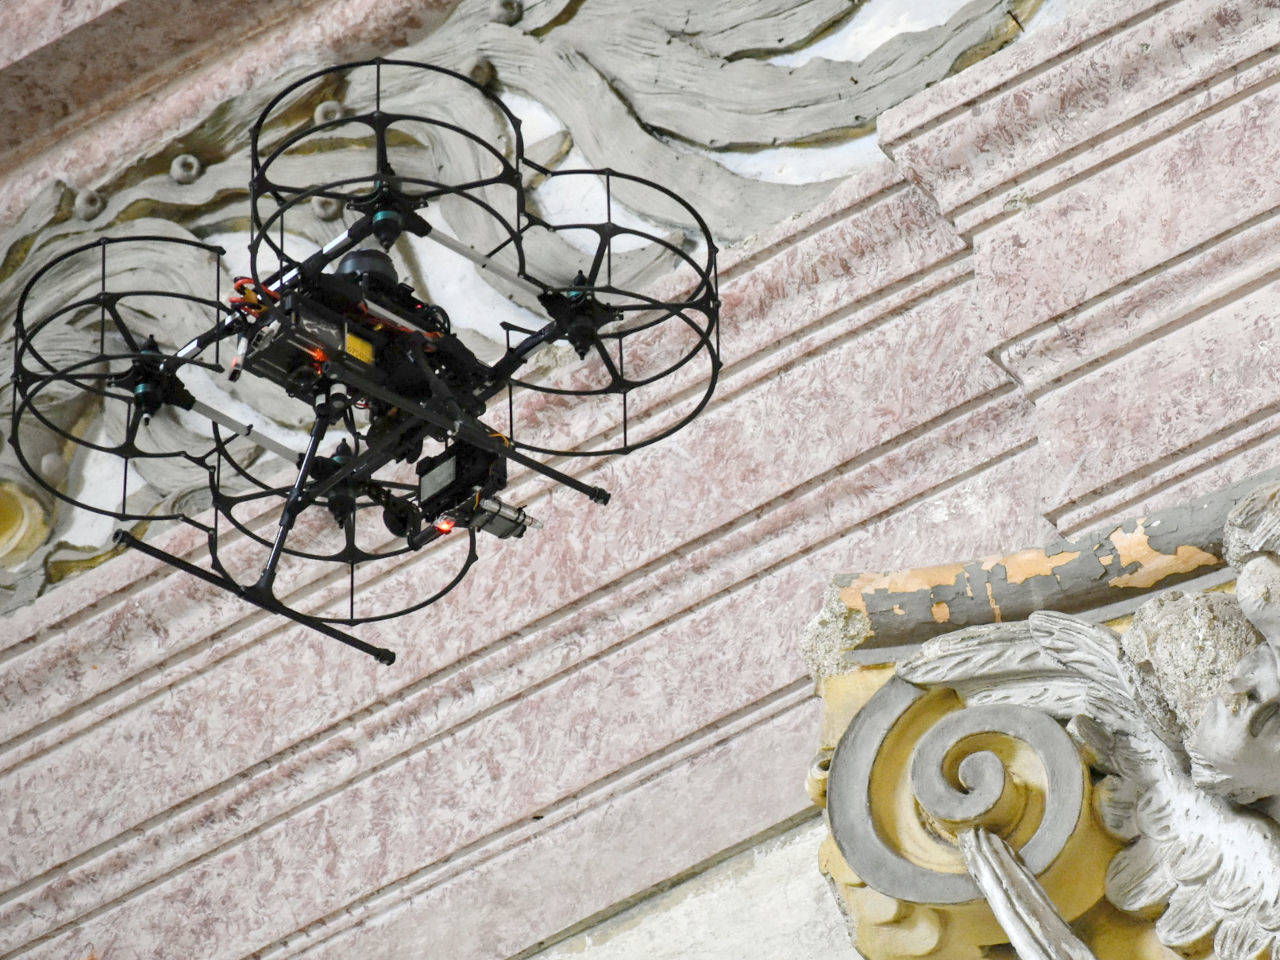
\includegraphics[width=0.235\textwidth]{./fig/photos/dronument_2_2_1-5.jpg}};
    \begin{scope}[x={(a.south east)},y={(a.north west)}]
      %%{ grid
      % % useful grid to help you find coordinates for plotting the overlay
      % \draw[black, xstep=.1, ystep=.1] (0,0) grid (1,1);
      % \foreach \i in {0,0.1,0.2,0.3,0.4,0.5,0.6,0.7,0.8,0.9,1} {
      %   \node[align=center] at (\i, -0.05) {\i};
      %   \node[align=center] at (\i, 1.05) {\i};
      %   \node[align=center] at (-0.05, \i) {\i};
      %   \node[align=center] at (1.05, \i) {\i};
      % }
      %%}
      % plot some stuff over the image
      \fill[white] (0.001, 0.001) rectangle (0.12,0.13);
      \fill[draw=black, draw opacity=0.5, fill opacity=0] (0,0) rectangle (1, 1);
      \node[imgletter,text=black] (label) at (a.south west) {(a)};
    \end{scope}
  \end{tikzpicture}}
  \hfill%
  \subfloat {\begin{tikzpicture}
    \node[anchor=south west,inner sep=0] (a) at (0,0) { 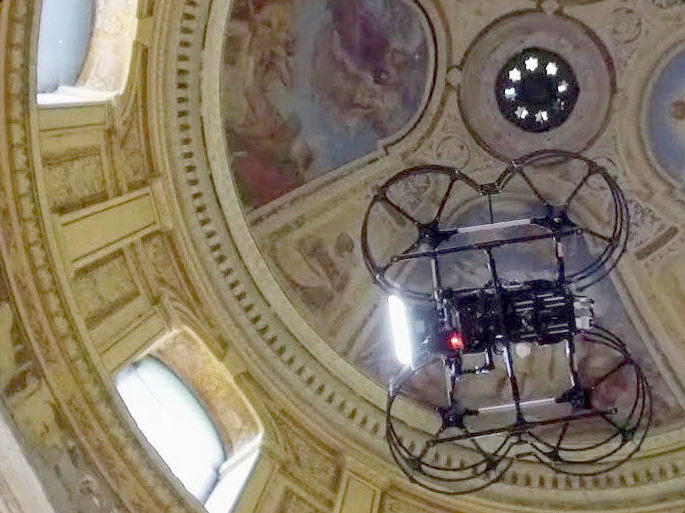
\includegraphics[width=0.235\textwidth]{./fig/photos/dronument_2_1-5.jpg}};
    \begin{scope}[x={(a.south east)},y={(a.north west)}]
      %%{ grid
      % % useful grid to help you find coordinates for plotting the overlay
      % \draw[black, xstep=.1, ystep=.1] (0,0) grid (1,1);
      % \foreach \i in {0,0.1,0.2,0.3,0.4,0.5,0.6,0.7,0.8,0.9,1} {
      %   \node[align=center] at (\i, -0.05) {\i};
      %   \node[align=center] at (\i, 1.05) {\i};
      %   \node[align=center] at (-0.05, \i) {\i};
      %   \node[align=center] at (1.05, \i) {\i};
      % }
      %%}
      % plot some stuff over the image
      \fill[white] (0.001, 0.001) rectangle (0.12,0.13);
      \fill[draw=black, draw opacity=0.5, fill opacity=0] (0,0) rectangle (1, 1);
      \node[imgletter,text=black] (label) at (a.south west) {(b)};
    \end{scope}
  \end{tikzpicture}}
  \caption{An inspection of an indoor historical building is conducted (a) to monitor the state of frescoes, and (b) to assess the state of wall paintings.}
  \label{fig:dronument}
\end{figure}

%%}

%%}

%%{ Sec: UAV swarms and formations

\section{UAV swarms and formations}
\label{sec:uav_swarms_and_formations}

%%{ Fig: swamrs

\begin{figure}
  \centering
  \subfloat {\begin{tikzpicture}
    \node[anchor=south west,inner sep=0] (a) at (0,0) { 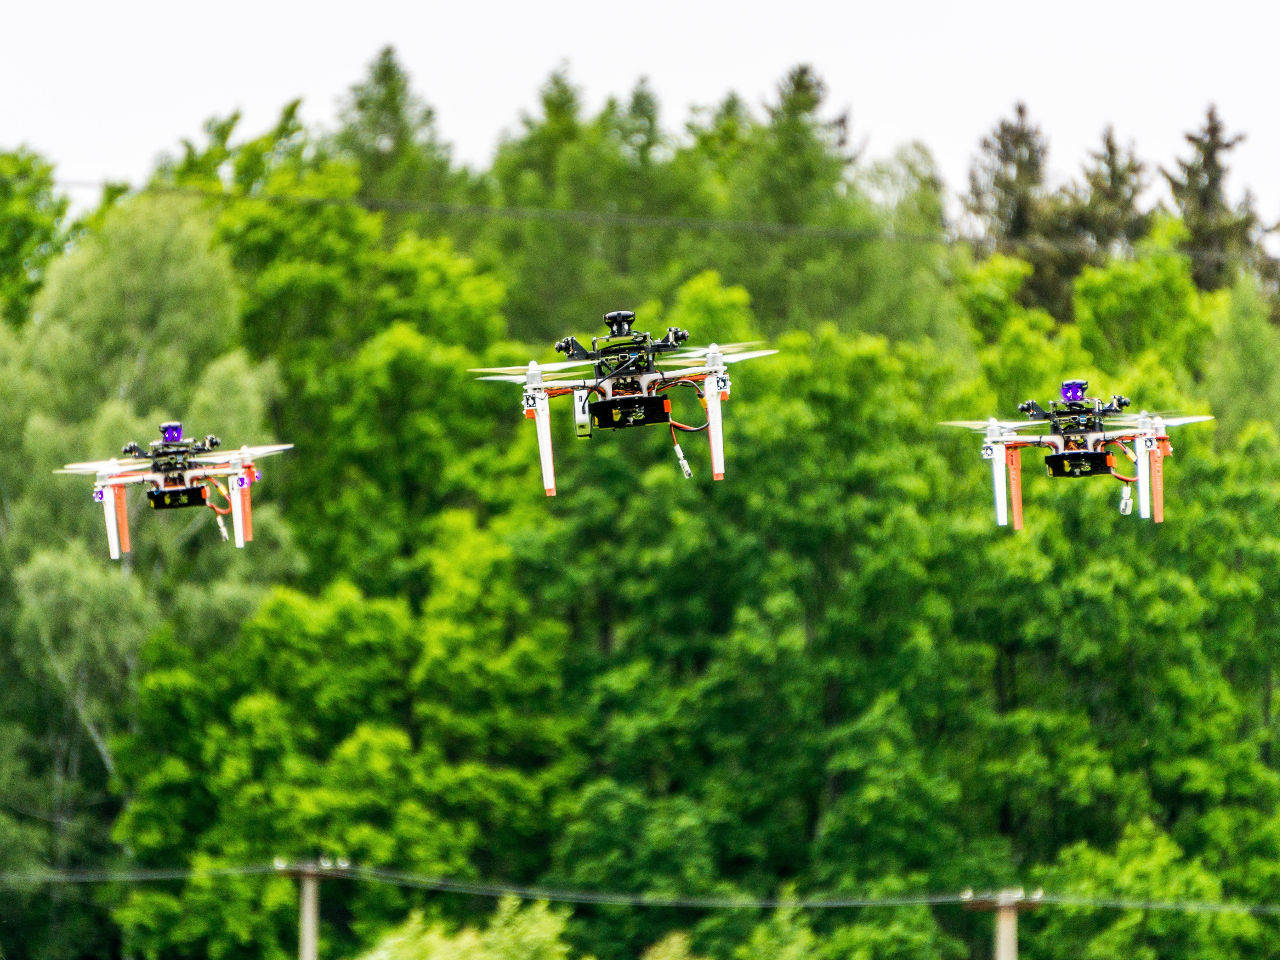
\includegraphics[width=0.235\textwidth]{./fig/photos/swarm_2_1-5.jpg}};
    \begin{scope}[x={(a.south east)},y={(a.north west)}]
      %%{ grid
      % % useful grid to help you find coordinates for plotting the overlay
      % \draw[black, xstep=.1, ystep=.1] (0,0) grid (1,1);
      % \foreach \i in {0,0.1,0.2,0.3,0.4,0.5,0.6,0.7,0.8,0.9,1} {
      %   \node[align=center] at (\i, -0.05) {\i};
      %   \node[align=center] at (\i, 1.05) {\i};
      %   \node[align=center] at (-0.05, \i) {\i};
      %   \node[align=center] at (1.05, \i) {\i};
      % }
      %%}
      \fill[white] (0.001, 0.001) rectangle (0.12,0.13);
      % plot some stuff over the image
      \fill[draw=black, draw opacity=0.5, fill opacity=0] (0,0) rectangle (1, 1);
      \node[imgletter,text=black] (label) at (a.south west) {(a)};
    \end{scope}
  \end{tikzpicture}}
  \hfill
  \subfloat {\begin{tikzpicture}
    \node[anchor=south west,inner sep=0] (a) at (0,0) { 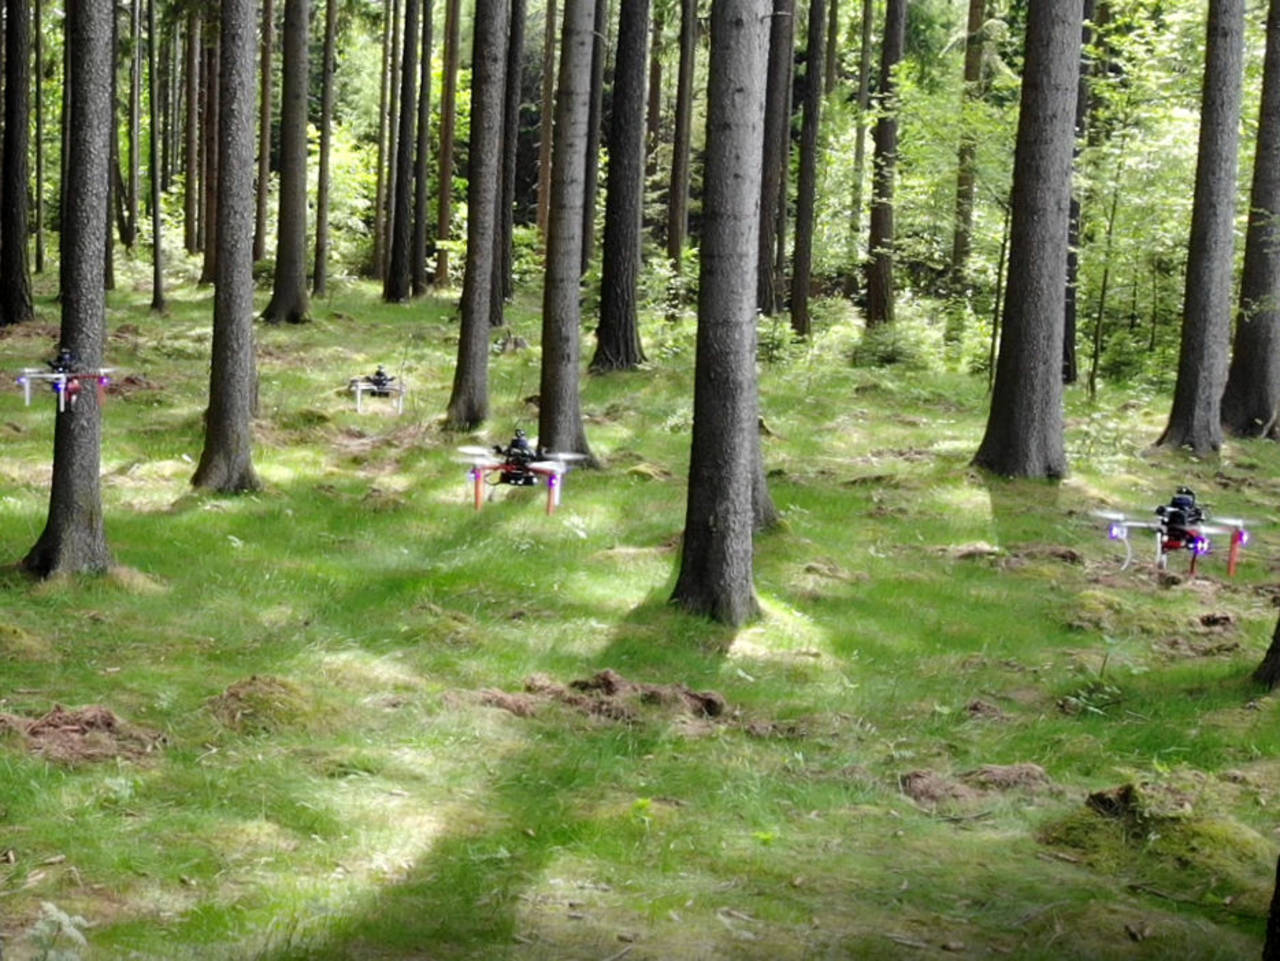
\includegraphics[width=0.235\textwidth]{./fig/photos/swarm_forest_2_1-5.jpg}};
    \begin{scope}[x={(a.south east)},y={(a.north west)}]
      %%{ grid
      % useful grid to help you find coordinates for plotting the overlay
      % \draw[black, xstep=.1, ystep=.1] (0,0) grid (1,1);
      % \foreach \i in {0,0.1,0.2,0.3,0.4,0.5,0.6,0.7,0.8,0.9,1} {
      %   \node[align=center] at (\i, -0.05) {\i};
      %   \node[align=center] at (\i, 1.05) {\i};
      %   \node[align=center] at (-0.05, \i) {\i};
      %   \node[align=center] at (1.05, \i) {\i};
      % }
      %%}

      \draw[->, white, thick] (0.45, 0.20) -- (0.07, 0.57);
      \draw[->, white, thick] (0.45, 0.20) -- (0.30, 0.55);
      \draw[->, white, thick] (0.45, 0.20) -- (0.40, 0.45);
      \draw[->, white, thick] (0.45, 0.20) -- (0.85, 0.40);
      \draw (0.45,0.15) node [text=white] {\small UAVs};

      \fill[white] (0.001, 0.001) rectangle (0.12,0.13);
      % plot some stuff over the image
      \fill[draw=black, draw opacity=0.5, fill opacity=0] (0,0) rectangle (1, 1);
      \node[imgletter,text=black] (label) at (a.south west) {(b)};
    \end{scope}
  \end{tikzpicture}}
  \caption{Swarms of multirotor \acp{UAV} testing novel flocking algorithms while localized (a) by a \ac{GNSS} system, and (b) by onboard sensors only within a forest environment.}
  \label{fig:swarms}
\end{figure}

%%}

%%}

%%{ Sec: The DARPA Subterranean (SubT) challenge

\section{The DARPA Subterranean (SubT) challenge}

%%{ Fig: DARPA SubT

\begin{figure}
  \centering
  \subfloat {\begin{tikzpicture}
    \node[anchor=south west,inner sep=0] (a) at (0,0) { 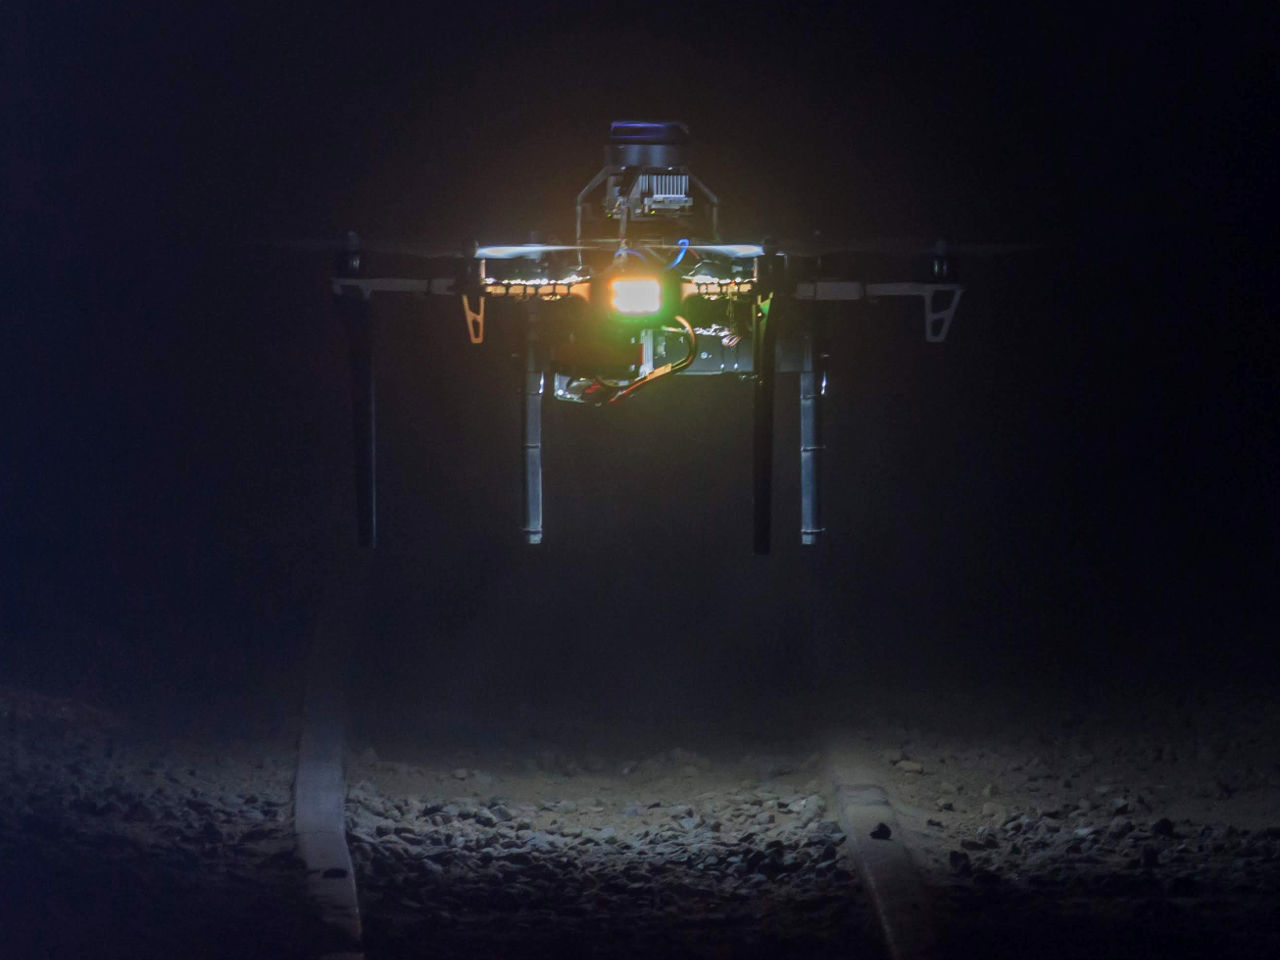
\includegraphics[width=0.235\textwidth]{./fig/photos/darpa_stix_2_1-5.jpg}};
    \begin{scope}[x={(a.south east)},y={(a.north west)}]
      %%{ grid
      % % useful grid to help you find coordinates for plotting the overlay
      % \draw[black, xstep=.1, ystep=.1] (0,0) grid (1,1);
      % \foreach \i in {0,0.1,0.2,0.3,0.4,0.5,0.6,0.7,0.8,0.9,1} {
      %   \node[align=center] at (\i, -0.05) {\i};
      %   \node[align=center] at (\i, 1.05) {\i};
      %   \node[align=center] at (-0.05, \i) {\i};
      %   \node[align=center] at (1.05, \i) {\i};
      % }
      %%}
      % plot some stuff over the image
      \fill[white] (0.001, 0.001) rectangle (0.12,0.13);
      \fill[draw=black, draw opacity=0.5, fill opacity=0] (0,0) rectangle (1, 1);
      \node[imgletter,text=black] (label) at (a.south west) {(a)};
    \end{scope}
  \end{tikzpicture}}
  \hfill%
  \subfloat {\begin{tikzpicture}
    \node[anchor=south west,inner sep=0] (a) at (0,0) { 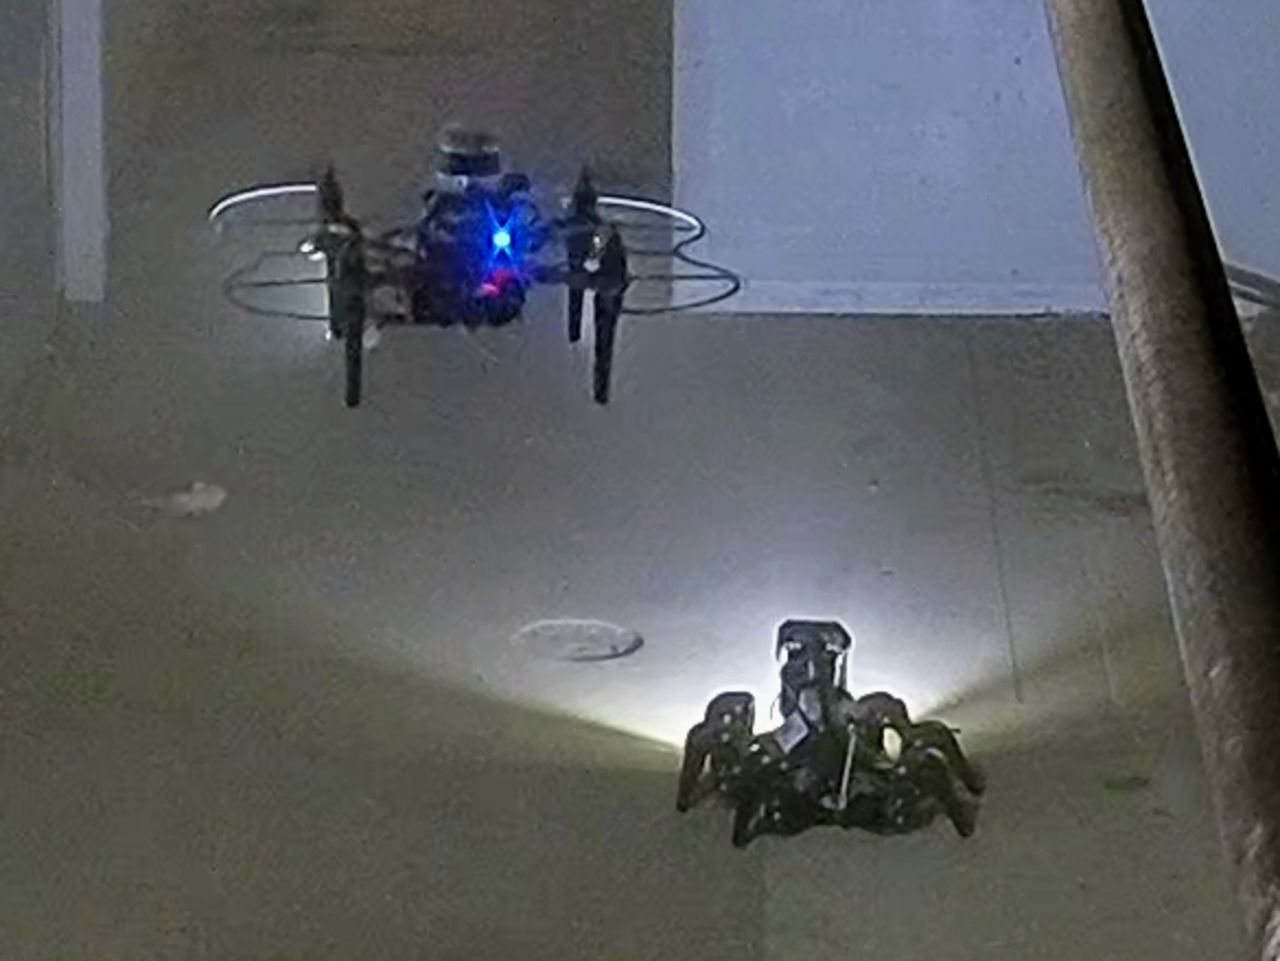
\includegraphics[width=0.235\textwidth]{./fig/photos/darpa_drone_beta_2_1-5.jpg}};
    \begin{scope}[x={(a.south east)},y={(a.north west)}]
      %%{ grid
      % % useful grid to help you find coordinates for plotting the overlay
      % \draw[black, xstep=.1, ystep=.1] (0,0) grid (1,1);
      % \foreach \i in {0,0.1,0.2,0.3,0.4,0.5,0.6,0.7,0.8,0.9,1} {
      %   \node[align=center] at (\i, -0.05) {\i};
      %   \node[align=center] at (\i, 1.05) {\i};
      %   \node[align=center] at (-0.05, \i) {\i};
      %   \node[align=center] at (1.05, \i) {\i};
      % }
      %%}
      % plot some stuff over the image
      \fill[white] (0.001, 0.001) rectangle (0.12,0.13);
      \fill[draw=black, draw opacity=0.5, fill opacity=0] (0,0) rectangle (1, 1);
      \node[imgletter,text=black] (label) at (a.south west) {(b)};
    \end{scope}
  \end{tikzpicture}}
  \caption{Unmanned Aerial Vehicles during the \ac{DARPA} SubT challenge. The photos depict (a) a \ac{UAV} exploring an underground mine, and (b) mapping an unfinished nuclear power plant.}
  \label{fig:darpa}
\end{figure}

%%}

%%}

%%{ Sec: MBZIRC 2017 competition

\section{MBZIRC 2017 competition}

\fullciteinbox{baca2019autonomous}{}
\fullciteinbox{loianno2018localization}{}

%%{ Fig: MBZIRC 2017

\begin{figure}
  \centering
  \subfloat {\begin{tikzpicture}
    \node[anchor=south west,inner sep=0] (a) at (0,0) { 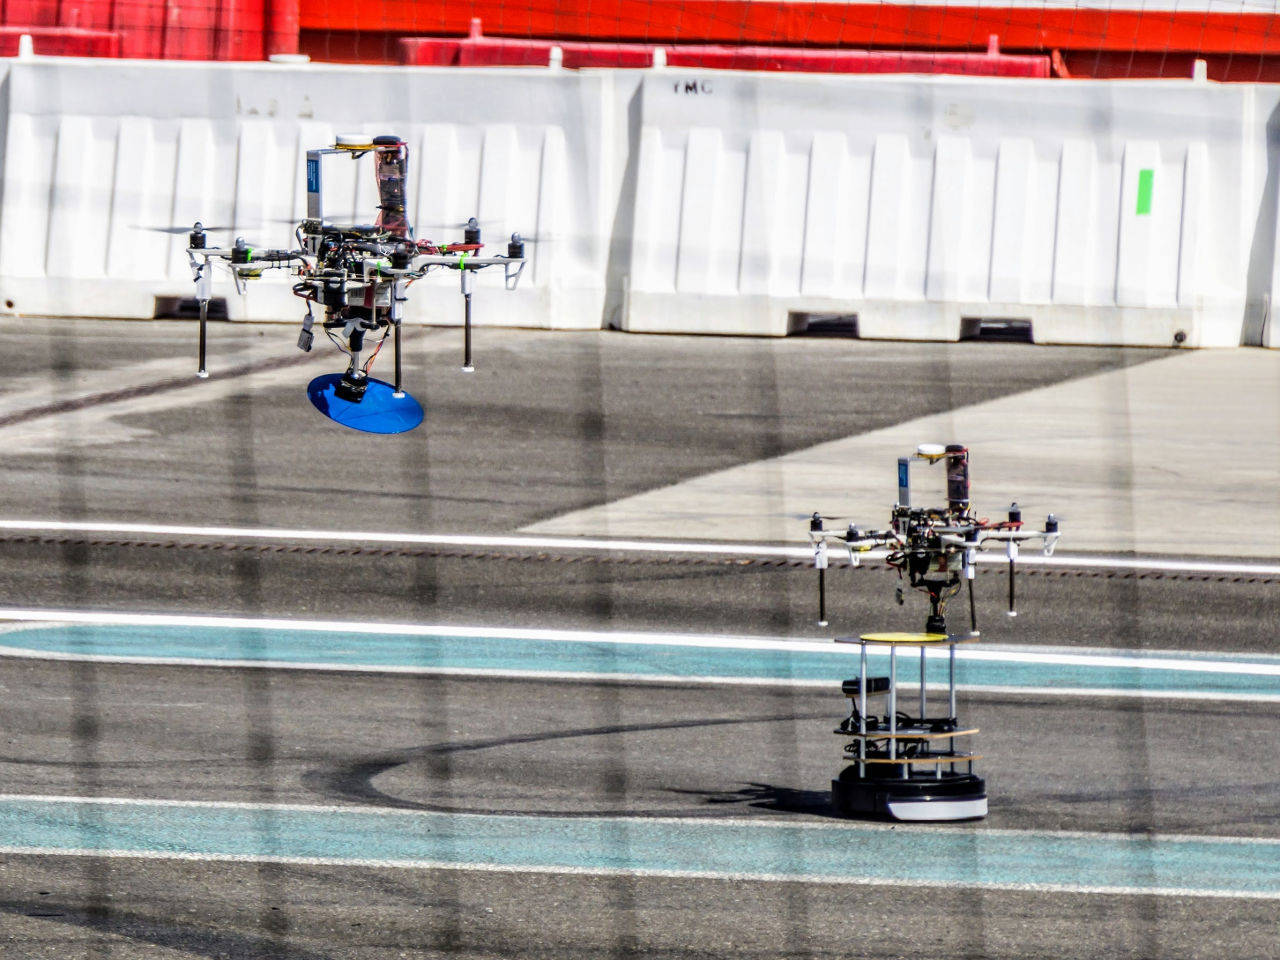
\includegraphics[width=0.235\textwidth]{./fig/photos/grasping_2017_2_1-5.jpg}};
    \begin{scope}[x={(a.south east)},y={(a.north west)}]
      %%{ grid
      % % useful grid to help you find coordinates for plotting the overlay
      % \draw[black, xstep=.1, ystep=.1] (0,0) grid (1,1);
      % \foreach \i in {0,0.1,0.2,0.3,0.4,0.5,0.6,0.7,0.8,0.9,1} {
      %   \node[align=center] at (\i, -0.05) {\i};
      %   \node[align=center] at (\i, 1.05) {\i};
      %   \node[align=center] at (-0.05, \i) {\i};
      %   \node[align=center] at (1.05, \i) {\i};
      % }
      %%}
      % plot some stuff over the image
      \fill[white] (0.001, 0.001) rectangle (0.12,0.13);
      \fill[draw=black, draw opacity=0.5, fill opacity=0] (0,0) rectangle (1, 1);
      \node[imgletter,text=black] (label) at (a.south west) {(a)};
    \end{scope}
  \end{tikzpicture}}
  \hfill%
  \subfloat {\begin{tikzpicture}
    \node[anchor=south west,inner sep=0] (a) at (0,0) { 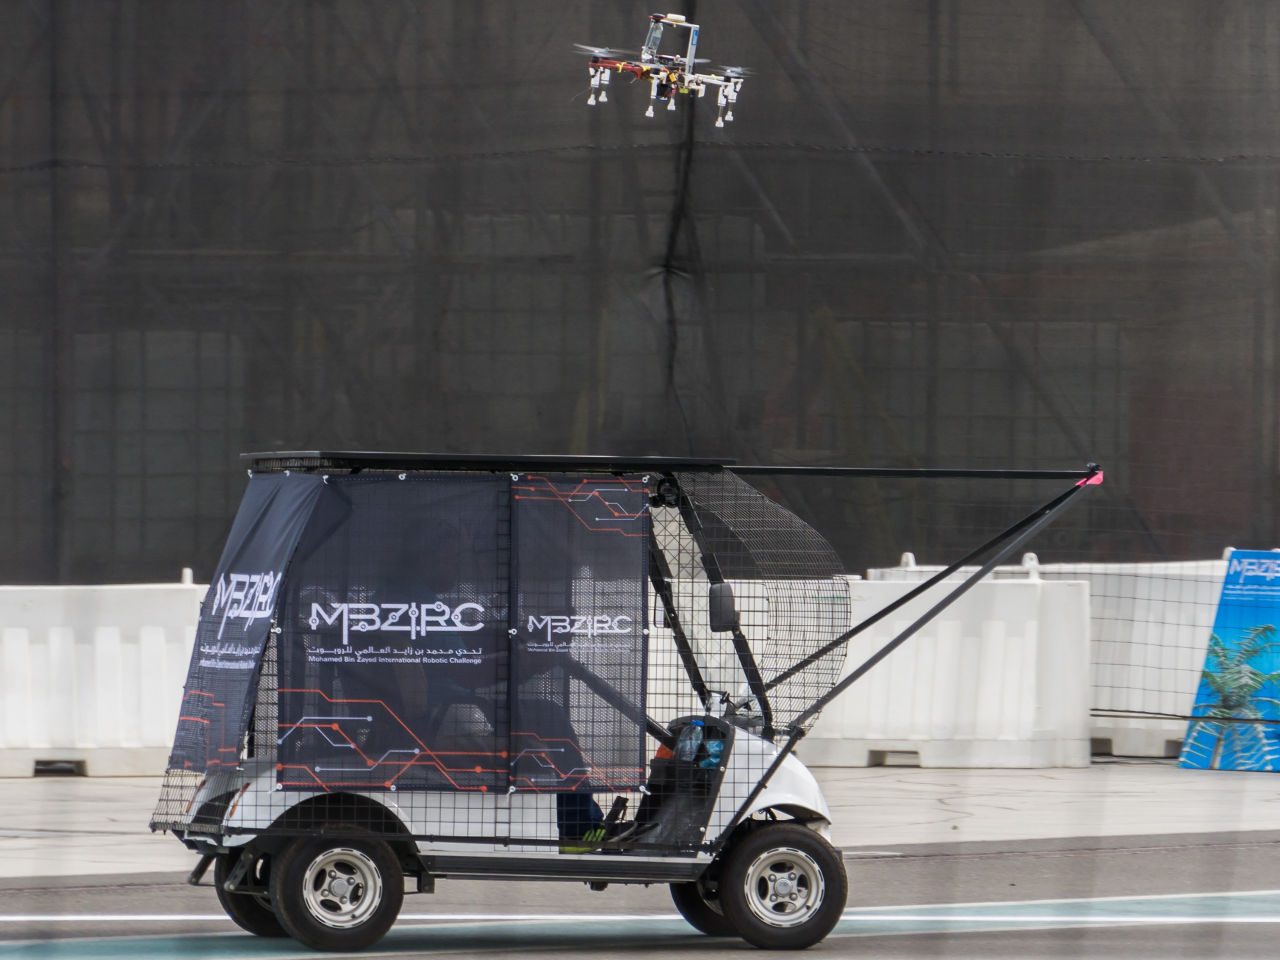
\includegraphics[width=0.235\textwidth]{./fig/photos/landing_2017_2_1-5.jpg}};
    \begin{scope}[x={(a.south east)},y={(a.north west)}]
      %%{ grid
      % % useful grid to help you find coordinates for plotting the overlay
      % \draw[black, xstep=.1, ystep=.1] (0,0) grid (1,1);
      % \foreach \i in {0,0.1,0.2,0.3,0.4,0.5,0.6,0.7,0.8,0.9,1} {
      %   \node[align=center] at (\i, -0.05) {\i};
      %   \node[align=center] at (\i, 1.05) {\i};
      %   \node[align=center] at (-0.05, \i) {\i};
      %   \node[align=center] at (1.05, \i) {\i};
      % }
      %%}
      % plot some stuff over the image
      \fill[white] (0.001, 0.001) rectangle (0.12,0.13);
      \fill[draw=black, draw opacity=0.5, fill opacity=0] (0,0) rectangle (1, 1);
      \node[imgletter,text=black] (label) at (a.south west) {(b)};
    \end{scope}
  \end{tikzpicture}}
  \caption{The CTU-UPENN-UoL team during the MBZIRC 2017 competition. The photos show (a) two \acp{UAV} while delivering ferrous objects, and (b) a \ac{UAV} during autonomous landing on a moving car.}
  \label{fig:mbzirc_2017}
\end{figure}

%%}

%%}

%%{ Sec: MBZIRC 2020 competition

\section{MBZIRC 2020 competition}

%%{ Fig: MBZIRC 2020

\begin{figure}
  \centering
  \subfloat {\begin{tikzpicture}
    \node[anchor=south west,inner sep=0] (a) at (0,0) { 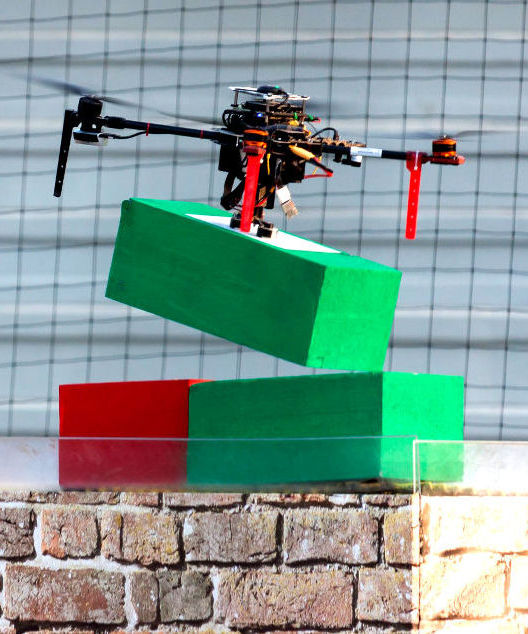
\includegraphics[width=0.155\textwidth]{./fig/photos/brick_placing_1-25_1-5.jpg}};
    \begin{scope}[x={(a.south east)},y={(a.north west)}]
      %%{ grid
      % % useful grid to help you find coordinates for plotting the overlay
      % \draw[black, xstep=.1, ystep=.1] (0,0) grid (1,1);
      % \foreach \i in {0,0.1,0.2,0.3,0.4,0.5,0.6,0.7,0.8,0.9,1} {
      %   \node[align=center] at (\i, -0.05) {\i};
      %   \node[align=center] at (\i, 1.05) {\i};
      %   \node[align=center] at (-0.05, \i) {\i};
      %   \node[align=center] at (1.05, \i) {\i};
      % }
      %%}
      % plot some stuff over the image
      \fill[white] (0.001, 0.001) rectangle (0.18,0.13);
      \fill[draw=black, draw opacity=0.5, fill opacity=0] (0,0) rectangle (1, 1);
      \node[imgletter,text=black] (label) at (a.south west) {(a)};
    \end{scope}
  \end{tikzpicture}}
  \hfill%
  \subfloat {\begin{tikzpicture}
    \node[anchor=south west,inner sep=0] (a) at (0,0) { 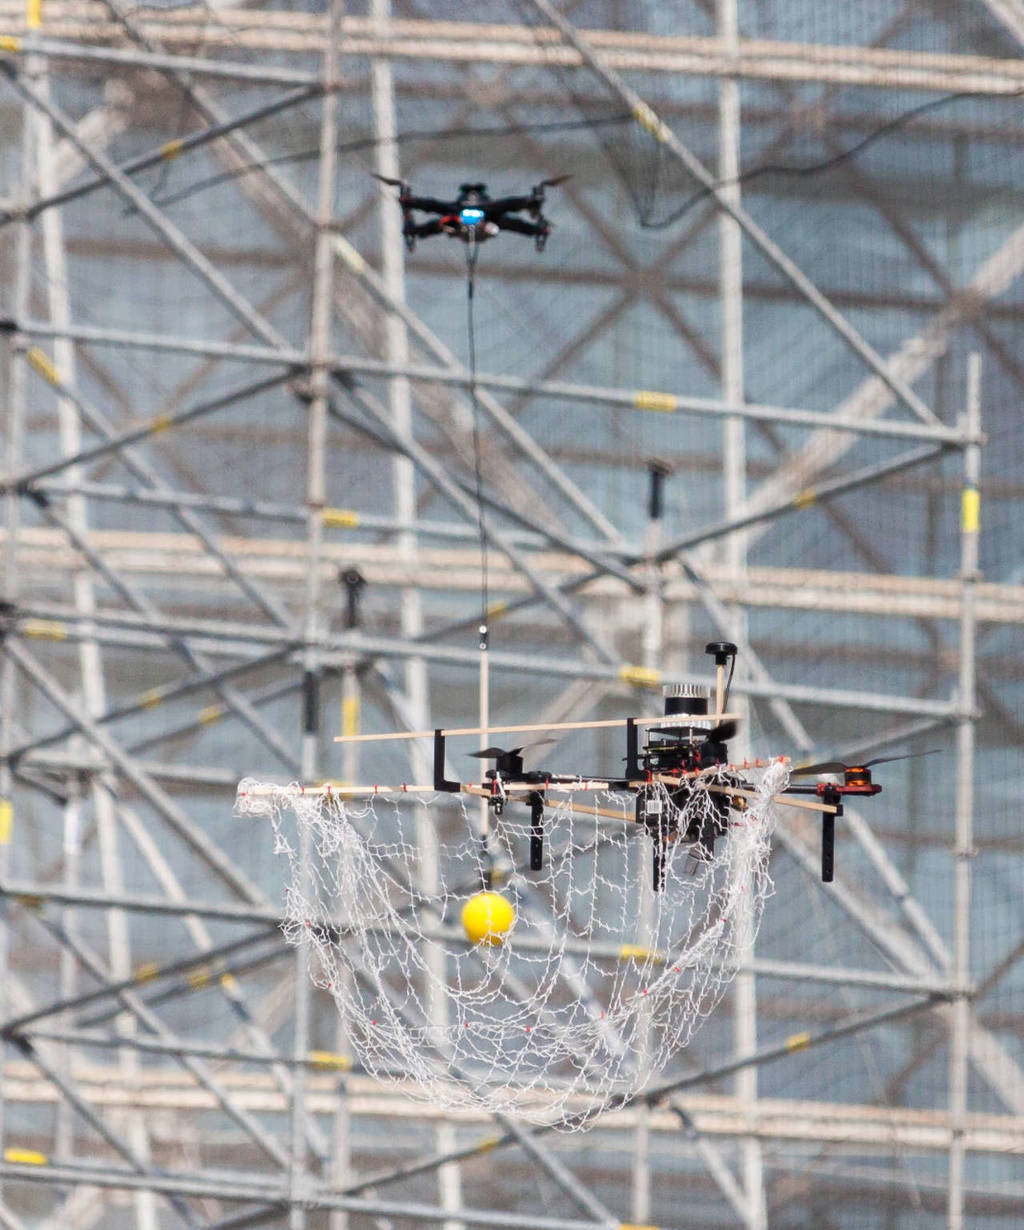
\includegraphics[width=0.155\textwidth]{./fig/photos/ball_catching_1-25_1-5.jpg}};
    \begin{scope}[x={(a.south east)},y={(a.north west)}]
      %%{ grid
      % % useful grid to help you find coordinates for plotting the overlay
      % \draw[black, xstep=.1, ystep=.1] (0,0) grid (1,1);
      % \foreach \i in {0,0.1,0.2,0.3,0.4,0.5,0.6,0.7,0.8,0.9,1} {
      %   \node[align=center] at (\i, -0.05) {\i};
      %   \node[align=center] at (\i, 1.05) {\i};
      %   \node[align=center] at (-0.05, \i) {\i};
      %   \node[align=center] at (1.05, \i) {\i};
      % }
      %%}
      % plot some stuff over the image
      \fill[white] (0.001, 0.001) rectangle (0.18,0.13);
      \fill[draw=black, draw opacity=0.5, fill opacity=0] (0,0) rectangle (1, 1);
      \node[imgletter,text=black] (label) at (a.south west) {(b)};
    \end{scope}
  \end{tikzpicture}}
  \hfill%
  \subfloat {\begin{tikzpicture}
    \node[anchor=south west,inner sep=0] (a) at (0,0) { 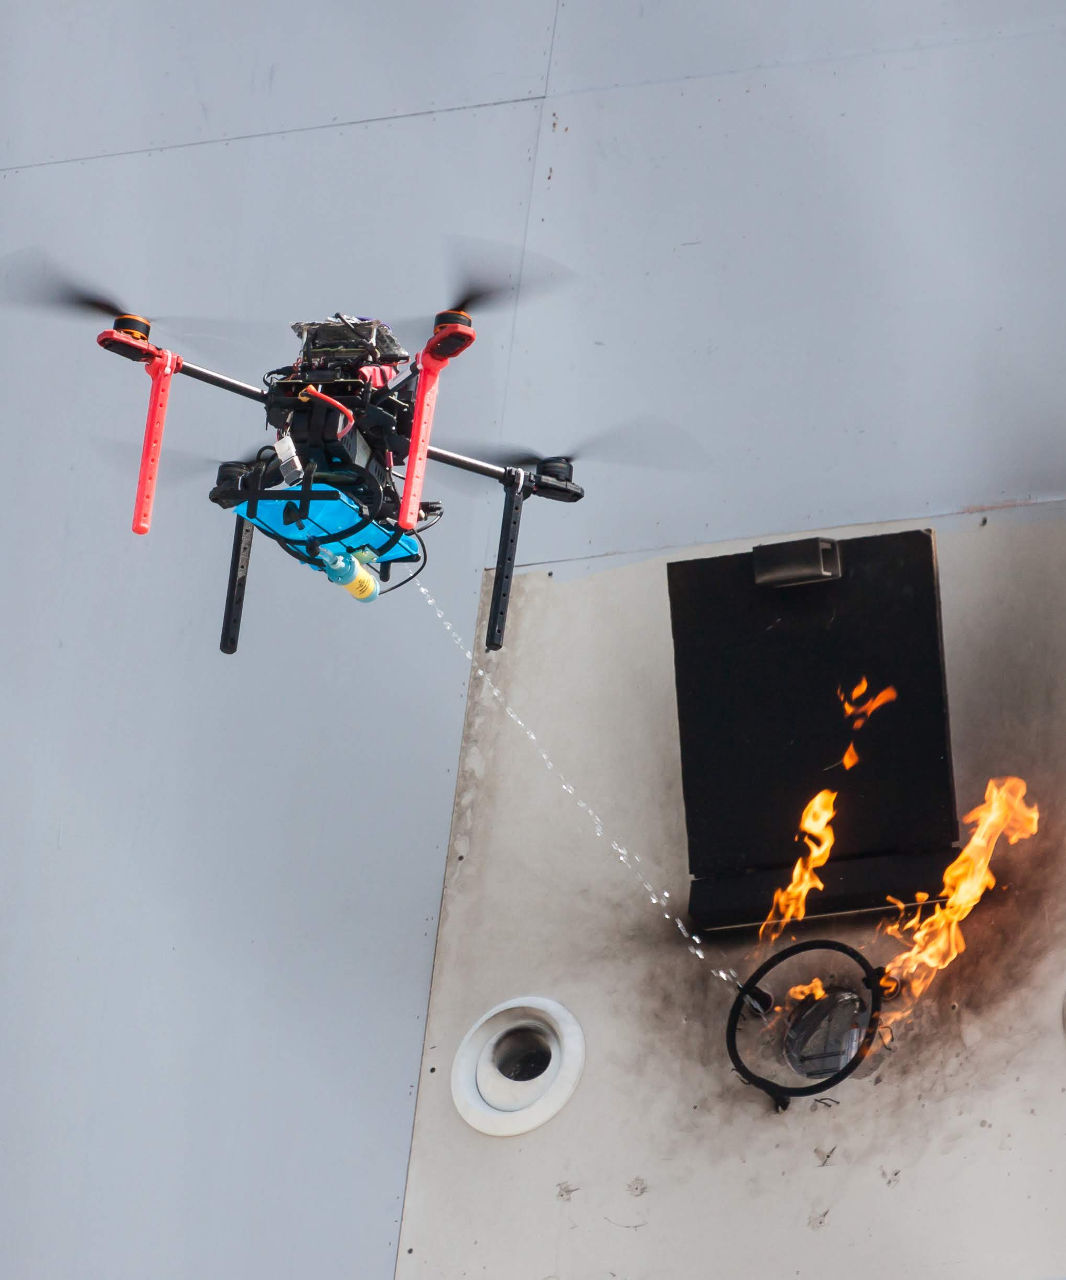
\includegraphics[width=0.155\textwidth]{./fig/photos/ext_1-25_1-5.jpg}};
    \begin{scope}[x={(a.south east)},y={(a.north west)}]
      %%{ grid
      % % useful grid to help you find coordinates for plotting the overlay
      % \draw[black, xstep=.1, ystep=.1] (0,0) grid (1,1);
      % \foreach \i in {0,0.1,0.2,0.3,0.4,0.5,0.6,0.7,0.8,0.9,1} {
      %   \node[align=center] at (\i, -0.05) {\i};
      %   \node[align=center] at (\i, 1.05) {\i};
      %   \node[align=center] at (-0.05, \i) {\i};
      %   \node[align=center] at (1.05, \i) {\i};
      % }
      %%}
      % plot some stuff over the image
      \fill[white] (0.001, 0.001) rectangle (0.18,0.13);
      \fill[draw=black, draw opacity=0.5, fill opacity=0] (0,0) rectangle (1, 1);
      \node[imgletter,text=black] (label) at (a.south west) {(c)};
    \end{scope}
  \end{tikzpicture}}\\
  \vspace{-0.8em}
  \subfloat {\begin{tikzpicture}
    \node[anchor=south west,inner sep=0] (a) at (0,0) { 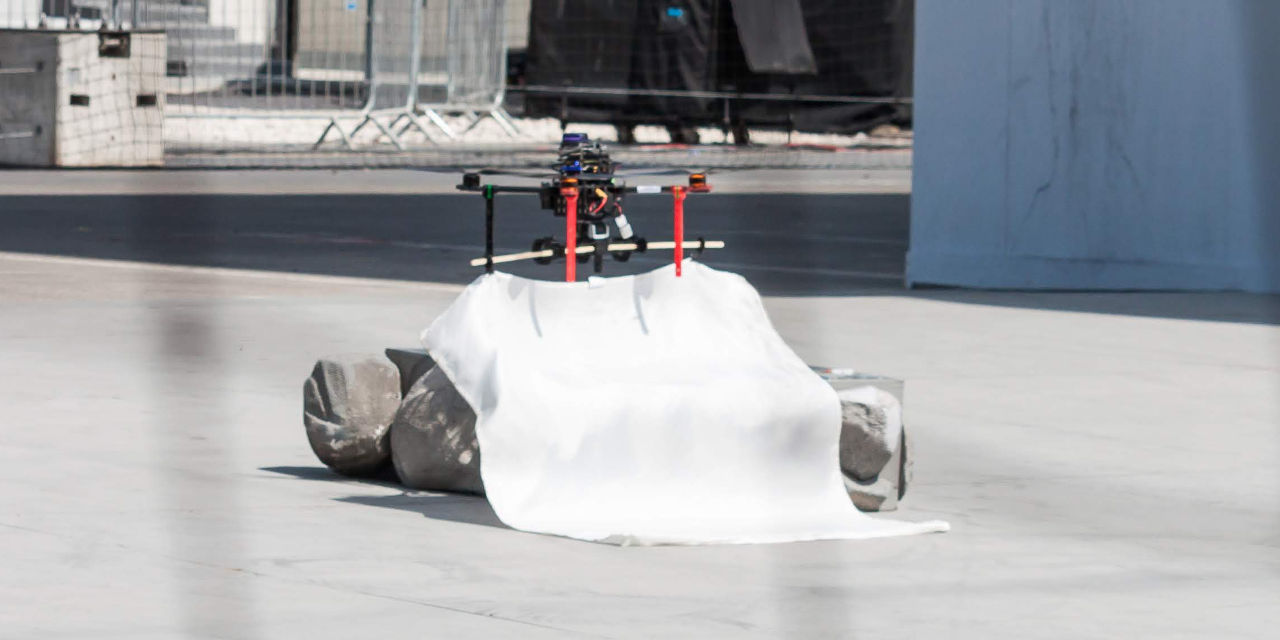
\includegraphics[width=0.235\textwidth]{./fig/photos/blanket_2_1.jpg}};
    \begin{scope}[x={(a.south east)},y={(a.north west)}]
      %%{ grid
      % % useful grid to help you find coordinates for plotting the overlay
      % \draw[black, xstep=.1, ystep=.1] (0,0) grid (1,1);
      % \foreach \i in {0,0.1,0.2,0.3,0.4,0.5,0.6,0.7,0.8,0.9,1} {
      %   \node[align=center] at (\i, -0.05) {\i};
      %   \node[align=center] at (\i, 1.05) {\i};
      %   \node[align=center] at (-0.05, \i) {\i};
      %   \node[align=center] at (1.05, \i) {\i};
      % }
      %%}
      % plot some stuff over the image
      \fill[white] (0.001, 0.001) rectangle (0.13,0.20);
      \fill[draw=black, draw opacity=0.5, fill opacity=0] (0,0) rectangle (1, 1);
      \node[imgletter,text=black] (label) at (a.south west) {(d)};
    \end{scope}
  \end{tikzpicture}}
  \hfill%
  \subfloat {\begin{tikzpicture}
    \node[anchor=south west,inner sep=0] (a) at (0,0) { 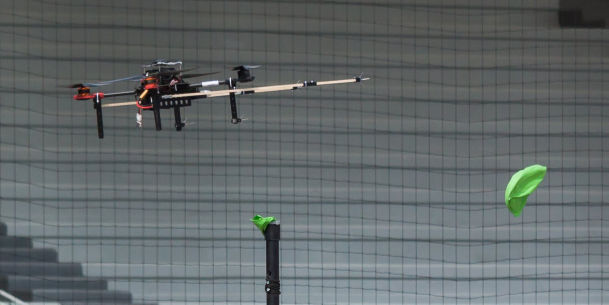
\includegraphics[width=0.235\textwidth]{./fig/photos/popping_2_1.jpg}};
    \begin{scope}[x={(a.south east)},y={(a.north west)}]
      %%{ grid
      % % useful grid to help you find coordinates for plotting the overlay
      % \draw[black, xstep=.1, ystep=.1] (0,0) grid (1,1);
      % \foreach \i in {0,0.1,0.2,0.3,0.4,0.5,0.6,0.7,0.8,0.9,1} {
      %   \node[align=center] at (\i, -0.05) {\i};
      %   \node[align=center] at (\i, 1.05) {\i};
      %   \node[align=center] at (-0.05, \i) {\i};
      %   \node[align=center] at (1.05, \i) {\i};
      % }
      %%}
      % plot some stuff over the image
      \fill[white] (0.001, 0.001) rectangle (0.13,0.20);
      \fill[draw=black, draw opacity=0.5, fill opacity=0] (0,0) rectangle (1, 1);
      \node[imgletter,text=black] (label) at (a.south west) {(e)};
    \end{scope}
  \end{tikzpicture}}
  \caption{The CTU-UPENN-NYU team during the MBZIRC 2020 competition. The photos depict (a) autonomous wall building, (b) autonomous ball catching, (c) autonomous fire extinguishing, (d) autonomous fire blanket deployment, and (e) autonomous balloon popping.}
  \label{fig:mbzirc_2020}
\end{figure}

%%}

%%}

% INCLUDE THE FOLLOWING PDFS
\includepaper{loianno2018localization}
\includepaper{baca2019autonomous}

%%}

%% | ------------------------ Chapter 5 ----------------------- |

%%{ Ionizing Radiation Detection and Localization by UAVs

\chapternoclear{Ionizing Radiation Detection and Localization by UAVs}
\chaptermark{Ionizing Radiation Sources Localization}

Ongoing research realized in the accepted TACR 2020-2022 project FW01010317:\\
``\textit{Lokalizace zdrojů ionizující radiace pomocí malých bezpilotních helikoptér s detektorem na principu Comptonovy kamery}''.

Relevant author's publications (will be discussed):
\fullciteinbox{baca2016miniaturized}{}
\fullciteinbox{baca2018rospix}{}
\fullciteinbox{baca2018timepix}{}
\fullciteinbox{baca2019timepix}{}
\fullciteinbox{stibinger2020localization}{}

% INCLUDE THE FOLLOWING PDFs
\includepaper{baca2018timepix}
\includepaper{baca2019timepix}
\includepaper{stibinger2020localization}

%%}

%%}

%% | ------------------------ Chapter 6 ----------------------- |

%%{ Conclusion

\chapternoclear{Conclusion}

\todo{}

%%}

%% | ----------------------- References ----------------------- |

%%{ References

\appendix
\renewcommand\chaptername{Appendix}

\chapternoclear{References}

Below are listed all publications of the author.
Each citation is displayed with percentage contribution of the author and number of citations based on Web of Science~(WoS), Scopus and Google Scholar~(GS).
\todo{updated citations}

%%{ Core publications

\section{Thesis core publications}

\subsection*{Core articles in peer-reviewed journals}
\printbibliography[keyword={mine},keyword={phd_related},keyword={journal},keyword={core},notkeyword={submitted},heading=none,title={}]

\subsection*{Core conference proceedings}
\printbibliography[keyword={mine},keyword={phd_related},keyword={conference},keyword={core},notkeyword={submitted},heading=none,title={}]

\subsection*{Core articles --- submitted}
\printbibliography[keyword={mine},keyword={phd_related},keyword={submitted},keyword={core},heading=none,title={}]

%%}

%%{ Related publications

\section{Thesis-related author's publications}

\subsection*{Thesis-related articles in peer-reviewed journals}
\printbibliography[keyword={mine},keyword={phd_related},keyword={journal},notkeyword={core},notkeyword={submitted},heading=none,title={}]

% \subsection*{Thesis-related articles in peer-reviewed journals only with CiteScore~(CS)}
% \printbibliography[keyword={mine},keyword={phd_related},keyword={journal},keyword={cs},heading=none,title={}]

\subsection*{Thesis-related conference proceedings}
\printbibliography[keyword={mine},keyword={phd_related},keyword={conference},notkeyword={core},notkeyword={submitted},heading=none,title={}]

\subsection*{Thesis-related publications --- submitted}
\printbibliography[keyword={mine},keyword={phd_related},keyword={submitted},notkeyword={core},heading=none,title={}]

%%}

%%{ Partially-related publications

\section{Partially-related author's publications}

\subsection*{Partially-related articles in peer-reviewed journals}
\printbibliography[keyword={mine},keyword={phd_unrelated},keyword={journal},notkeyword={core},notkeyword={submitted},heading=none,title={}]

\subsection*{Partially-related conference proceedings}
\printbibliography[keyword={mine},keyword={phd_unrelated},keyword={conference},notkeyword={core},notkeyword={submitted},heading=none,title={}]

\subsection*{Partially-related publications --- submitted}
\printbibliography[keyword={mine},keyword={phd_unrelated},keyword={submitted},heading=none,title={}]

%%}

%%{ unrelated publications

\section{Unrelated author's publications}

\printbibliography[keyword={mine},notkeyword={phd_unrelated},notkeyword={phd_related},heading=none,title={}]

%%}

%%{ Cited references

\section{Cited references}
\printbibliography[notkeyword=mine,heading=none,title={}]

%%}

%%}

%% | ------------------------ Apendices ----------------------- |

%%{ Apendices

\appendix
\renewcommand\chaptername{Citations of author's publications}

\chapternoclear{Citations of author's publications}

Below are listed all citations of author's publications without self-citations.

\DeclareCiteCommand{\fullcite}
{\usebibmacro{prenote}}
{\clearfield{addendum}%
  \usedriver
  {\defcounter{minnames}{6}%
  \defcounter{maxnames}{6}}
{\thefield{entrytype}}}
{\multicitedelim}
{\usebibmacro{postnote}}

\noindent
\fullcite{saska2017system}
\begin{refsection}[citations/no_autocit/saska2017system.bib]
  \nocite{*}
  \printbibliography[heading=none,title={},env=favoritebib]
\end{refsection}

% \noindent
% \fullcite{faigl2017onsolution}
% \begin{refsection}[citations/no_autocit/faigl2017onsolution.bib]
%   \nocite{*}
%   \printbibliography[heading=none,title={},env=favoritebib]
% \end{refsection}

% \noindent
% \fullcite{saska2016formations}
% \begin{refsection}[citations/no_autocit/saska2016formations.bib]
%   \nocite{*}
%   \printbibliography[heading=none,title={},env=favoritebib]
% \end{refsection}

\noindent
\fullcite{baca2016miniaturized}
\begin{refsection}[citations/no_autocit/baca2016miniaturized.bib]
  \nocite{*}
  \printbibliography[heading=none,title={},env=favoritebib]
\end{refsection}

\noindent
\fullcite{loianno2018localization}
\begin{refsection}[citations/no_autocit/loianno2018localization.bib]
  \nocite{*}
  \printbibliography[heading=none,title={},env=favoritebib]
\end{refsection}

\noindent
\fullcite{spurny2019cooperative}
\begin{refsection}[citations/no_autocit/spurny2019cooperative.bib]
  \nocite{*}
  \printbibliography[heading=none,title={},env=favoritebib]
\end{refsection}

\noindent
\fullcite{daniel2016terrestrial}
\begin{refsection}[citations/no_autocit/daniel2016terrestrial.bib]
  \nocite{*}
  \printbibliography[heading=none,title={},env=favoritebib]
\end{refsection}

\noindent
\fullcite{baca2017autonomous}
\begin{refsection}[citations/no_autocit/baca2017autonomous.bib]
  \nocite{*}
  \printbibliography[heading=none,title={},env=favoritebib]
\end{refsection}

\noindent
\fullcite{baca2018model}
\begin{refsection}[citations/no_autocit/baca2018model.bib]
  \nocite{*}
  \printbibliography[heading=none,title={},env=favoritebib]
\end{refsection}

\noindent
\fullcite{daniel2017xray}
\begin{refsection}[citations/no_autocit/daniel2017xray.bib]
  \nocite{*}
  \printbibliography[heading=none,title={},env=favoritebib]
\end{refsection}

\noindent
\fullcite{urban2017vzlusat}
\begin{refsection}[citations/no_autocit/urban2017vzlusat.bib]
  \nocite{*}
  \printbibliography[heading=none,title={},env=favoritebib]
\end{refsection}

\noindent
\fullcite{baca2016embedded}
\begin{refsection}[citations/no_autocit/baca2016embedded.bib]
  \nocite{*}
  \printbibliography[heading=none,title={},env=favoritebib]
\end{refsection}

\noindent
\fullcite{baca2019autonomous}
\begin{refsection}[citations/no_autocit/baca2019autonomous.bib]
  \nocite{*}
  \printbibliography[heading=none,title={},env=favoritebib]
\end{refsection}

\noindent
\fullcite{saska2017documentation}
\begin{refsection}[citations/no_autocit/saska2017documentation.bib]
\nocite{*}
\printbibliography[heading=none,title={},env=favoritebib]
\end{refsection}

\noindent
\fullcite{giernacki2019realtime}
\begin{refsection}[citations/no_autocit/giernacki2019realtime.bib]
  \nocite{*}
  \printbibliography[heading=none,title={},env=favoritebib]
\end{refsection}

\noindent
\fullcite{chudoba2014localization}
\begin{refsection}[citations/no_autocit/chudoba2014localization.bib]
  \nocite{*}
  \printbibliography[heading=none,title={},env=favoritebib]
\end{refsection}

\noindent
\fullcite{saikin2020wildfire}
\begin{refsection}[citations/no_autocit/saikin2020wildfire.bib]
  \nocite{*}
  \printbibliography[heading=none,title={},env=favoritebib]
\end{refsection}

\noindent
\fullcite{daniel2019inorbit}
\begin{refsection}[citations/no_autocit/daniel2019inorbit.bib]
  \nocite{*}
  \printbibliography[heading=none,title={},env=favoritebib]
\end{refsection}

\noindent
\fullcite{baca2018timepix}
\begin{refsection}[citations/no_autocit/baca2018timepix.bib]
  \nocite{*}
  \printbibliography[heading=none,title={},env=favoritebib]
\end{refsection}

\noindent
\fullcite{baca2018rospix}
\begin{refsection}[citations/no_autocit/baca2018rospix.bib]
  \nocite{*}
  \printbibliography[heading=none,title={},env=favoritebib]
\end{refsection}

\noindent
\fullcite{spurny2016complex}
\begin{refsection}[citations/no_autocit/spurny2016complex.bib]
  \nocite{*}
  \printbibliography[heading=none,title={},env=favoritebib]
\end{refsection}

\noindent
\fullcite{chudoba2016exploration}
\begin{refsection}[citations/no_autocit/chudoba2016exploration.bib]
  \nocite{*}
  \printbibliography[heading=none,title={},env=favoritebib]
\end{refsection}

%%}

\end{document}
